\documentclass[10pt]{ctexart}

\usepackage{NotesTeXV3,lipsum}
%\usepackage{showframe}
\usepackage{amsmath}
\usepackage{amsfonts,amssymb}
\usepackage{mathrsfs}
\usepackage{tikz}
\usepackage{annotate-equations} % 公式标注美化
\usepackage{tikz-feynman}% 绘制费曼图 要使用LuaTex编译
%%%%%%%%%%%%%%%%%%%%%%%%%%%%%%%%%%%%%%%%%%%%%%%%%%%%%%%%%%%%%%%%%%%%%%%%
\usepackage{xfp} % higher precision (16 digits?)
\usepackage[outline]{contour} % glow around text
\usetikzlibrary{decorations.markings,decorations.pathmorphing}
\usetikzlibrary{angles,quotes} % for pic (angle labels)
\usetikzlibrary{arrows.meta} % for arrow size
\contourlength{1.4pt}
% tikz绘图一系列设定
\tikzset{>=latex} % for LaTeX arrow head
\colorlet{myred}{red!80!black}
\colorlet{myblue}{blue!80!black}
\colorlet{mygreen}{green!80!black}
\colorlet{mydarkred}{red!50!black}
\colorlet{mydarkblue}{blue!50!black}
\colorlet{mylightblue}{mydarkblue!6}
\colorlet{mypurple}{blue!40!red!80!black}
\colorlet{mydarkpurple}{blue!40!red!50!black}
\colorlet{mylightpurple}{mydarkpurple!80!red!6}
\colorlet{myorange}{orange!40!yellow!95!black}
\tikzstyle{cone}=[mydarkblue,line width=0.2,top color=blue!60!black!30,
bottom color=blue!60!black!50!red!30,shading angle=60,fill opacity=0.9]
\tikzstyle{cone back}=[mydarkblue,line width=0.1,dash pattern=on 1pt off 1pt]
\tikzstyle{world line}=[myblue!60,line width=0.4]
\tikzstyle{world line t}=[mypurple!60,line width=0.4]
\tikzstyle{particle}=[mygreen,line width=0.5]
\tikzstyle{photon}=[-{Latex[length=4,width=3]},myorange,line width=0.4,decorate,
decoration={snake,amplitude=0.9,segment length=4,post length=3.8}]
\tikzstyle{singularity}=[myred,line width=0.6,decorate,
decoration={zigzag,amplitude=2,segment length=6.17}]
\tikzset{declare function={%
		penrose(\x,\c)  = {\fpeval{2/pi*atan( (sqrt((1+tan(\x)^2)^2+4*\c*\c*tan(\x)^2)-1-tan(\x)^2) /(2*\c*tan(\x)^2) )}};%
		penroseu(\x,\t) = {\fpeval{atan(\x+\t)/pi+atan(\x-\t)/pi}};%
		penrosev(\x,\t) = {\fpeval{atan(\x+\t)/pi-atan(\x-\t)/pi}};%
		kruskal(\x,\c)  = {\fpeval{asin( \c*sin(2*\x) )*2/pi}};% Penrose coordinates for Kruskal
}}
\def\tick#1#2{\draw[thick] (#1) ++ (#2:0.04) --++ (#2-180:0.08)}
\def\Nsamples{40} % number samples in plot

% LIGHTCONE
\def\R{0.08} % size lightcone
\def\e{0.08} % vertical scale
\def\ang{45} % angle light cone
\def\angb{acos(sqrt(\e)*sin(\ang))} % angle ellipse center to point of tangency
\def\a{\R*sin(\ang)*sqrt(1-\e*sin(\ang)^2)/(1-\e*sin(\ang)^2)} % vertical radius
\def\b{\R*sqrt(\e)*sin(\ang)*cos(\ang)/(1-\e*sin(\ang)^2)} % horizontal radius
\def\coneback#1{ % light cone part to be drawn behind world lines
	\draw[cone back] % dashed line back
	(#1)++(-45:\R) arc({90-\angb}:{90+\angb}:{\a} and {\b});
	\draw[cone,shading angle=-60] % top edge & inside
	(#1)++(0,{\R*cos(\ang)/(1-\e*sin(\ang)^2)}) ellipse({\a} and {\b});
}
\def\conefront#1{ % light cone part to be drawn over world lines
	\draw[cone] % light cone outside
	(#1) --++ (45:\R) arc({\angb-90}:{-90-\angb}:{\a} and {\b})
	--++ (-45:2*\R) arc({90-\angb}:{-270+\angb}:{\a} and {\b}) -- cycle;
}
%%%%%%%%%%%%%%%%%%%%%%%%%%%%%%%%%%%%%%%%%%%%%%%%%%%%%%%%%%%%%%%%%%%%%%%%

\bibliographystyle{JHEP}

\begin{document}
	\title{{天球振幅科研笔记}\\{\normalsize{\itshape Celestial Amplitudes}}}
	\author{Bufan Zheng}
	\affiliation{
	Undergraduate Student at the Wuhan University\\
%	\href{https://adhumunt.github.io/}{Website}\\
%	\href{https://inspirehep.net/authors/1669979}{Inspire-HEP}\\
%	\href{https://www.linkedin.com/in/aditya-dhumuntarao-80a0b8112/}{LinkedIn}\\
	\href{https://github.com/WHUZBF}{GitHub}\\
	}
	\emailAdd{whuzbf@qq.com}
	\maketitle
	\newpage
	\pagestyle{fancynotes}
	\part{A quick review on SR \& GR}
\section{Basics conceptions in SR}\label{sec:1}
我们生活的空间是一个四维局部平坦的\textbf{Lorentz流形},也就是一个四维微分流形配备一个非正定、非退化的度规$g=g_{\mu\nu}dx^\mu\otimes dx^\nu$,这是一个$(0,2)$张量。局部平坦意思是说任何一点处都可以选取一个坐标系\sn{这个坐标系称为\textbf{局部惯性系},由于可以从指数映射结合测地线来构造这个惯性系,所以也称为\textbf{自由下落参考系}}使得$g_{\mu\nu}=\eta_{\mu\nu},\nabla_\rho g_{\mu\nu}$\sn{这里符号约定为$\eta_{\mu\nu}=(-,+,+,+)$}。而Lorentz体现在$\eta$有一个指标是负数,而且根据惯性定理,无论你选取什么坐标系将度规对角化,最终负数的个数都是一样的,这样一来我们便可以严格的区分时间和空间\sn{如果这里把$\eta$中的$-1$变成$+1$,我们称为\textbf{Riemann流形}}。

参数化流形后,时空上的每一点(事件)都将对应一个坐标$x^\mu$,时空中的曲线(世界线)可以参数化为$x^\mu(\tau)$,其可以看作是由矢量场$X=X^\mu\partial_\mu=\frac{x^\mu(\tau)}{d\tau}\partial_\mu$诱导的。考虑世界线上相邻的两点,我们可以定义线长为
\[dl=\sqrt{|g(X,X)|}=\int d\tau\sqrt{g_{\mu\nu}\frac{x^\mu}{d\tau}\frac{x^\nu}{d\tau}}\]
很多时候也把线长记为$ds^2=g_{\mu\nu}dx^\mu dx^\nu$但是在微分几何的严格意义下,$dx^\mu$是对偶矢量,并不是初等微积分中的微分,所以这个式子只能理解为$ds^2=g_{\mu\nu}dx^\mu\otimes dx^\nu$,也就是说$ds^2$只是张量$g$的另一个叫法而已!后面我们为了方便可能牺牲严谨性,使用$ds^2$表示世界线长。

GR中最重要的基本假设便是在坐标变换下物理定律是不变的,这说明作用量必须是标量,几乎唯一确定了真空引力场作用量为:
\begin{margintable}\footnotesize 
	\begin{tabularx}{\marginparwidth}{|X}
		$\Lambda$是宇宙学常数\\
		$g\equiv\det g_{\mu\nu}$\\
		$R$是Ricci标量\\
		取自然单位制$c=\hbar=1$
	\end{tabularx}
\end{margintable}
\begin{equation}
	S_{\mathrm{EH}}=\frac{1}{16\pi G}\int \mathrm{d}^4x\sqrt{-g} (R-2\Lambda)
\end{equation}
由于度规是张量,所以其在坐标变换下分量变换为:\sn{注意两边对应的自变量,因为张量都是关于流形上点的场,所以这里坐标变换后流形上某点对应的坐标也变了。}
\[\tilde{g}_{\mu\nu}(\tilde{x})=\frac{\partial \tilde{x}^\rho}{\partial x^\mu}\frac{\partial \tilde{x}^\sigma}{\partial x^\nu}g_{\rho\sigma}(x)\]
在SR中我们仅研究平直的时空,或者说只研究惯性系之间的变换,这些惯性系中的变换满足$\tilde{\eta}=\eta$,可以一般的记为:
\[\tilde{x}^\mu=\Lambda^{\mu}_{\ \nu}x^\nu+a^\mu\]
那么$\Lambda$满足:
\begin{equation}
	\Lambda^{\operatorname{T}}\eta\Lambda=\eta
\end{equation}
本笔记主要考虑SR时空。
\section{Poincar\'e group and Lorentz group}
显然所有的$\Lambda$构成了一个群,称之为\textbf{Lorentz群}:
\begin{equation}
	L\equiv O(3,1)\equiv\left\{\Lambda\in M(4,\mathbb{R})|	\Lambda^{\operatorname{T}}\eta\Lambda=\eta\right\}
\end{equation}
而所有的保度规变换还要加入$a^mu$,构成\textbf{Poincar\'e群}:$O(3,1)\ltimes \mathbb{R}$,群乘法为:
\begin{equation}
	(\Lambda,a)\cdot(\Lambda',a')=(\Lambda\cdot\Lambda',a+\Lambda\cdot a')
\end{equation}
利用Poincar\'e群的不等价不可约表示可以对基本粒子进行分类,见本部分末尾。后面我们将主要关注Lorentz群。
不难验证$\det \Lambda=\pm 1$,它将Lorentz群分成两个分支,其中$\det \Lambda=1$的部分含有单位元,构成子群\textbf{正规Lorentz群}。记为$SO(3,1)$或$L_+$

另外$(\Lambda^0_{\ 0})^2\geq 1$也将Lorentz群分成两个分支,其中$\Lambda^0_{\ 0}\geq1$的部分含有单位元,构成子群\textbf{正时Lorentz群}。记为$O(3,1)^\uparrow$或$L^\uparrow$。

最后$L^\uparrow_+\equiv L^\uparrow\cap L_+$也构成了$L$的一个子群。这些子群之间可以用时间反演和空间反演算符相联系:
\begin{equation}
	\mathcal{T}=\begin{pmatrix}
		-1&  &  & \\
		& 1 &  & \\
		&  & 1 & \\
		&  &  &1
	\end{pmatrix},\quad\quad\mathcal{P}=\begin{pmatrix}
	1&  &  & \\
	& -1 &  & \\
	&  & -1 & \\
	&  &  &-1
	\end{pmatrix}
\end{equation}
显然$L_+=\{L_+^\uparrow,\mathcal{T}\},L^\uparrow=\{L_+^\uparrow,\mathcal{P}\},L=\{L_+^\uparrow,\mathcal{T},\mathcal{P}\}$

\subsection{Poincar\'e algebra}
现在考虑群的局部性质,考虑无穷小坐标变换$x^\mu\mapsto x^\mu+\xi^\mu$,保度规条件为:
\begin{equation}\label{lie_eta}
	\mathscr{L}_\xi\eta_{\mu\nu}=\partial_\mu\xi_\nu+\partial_\mu\xi_\nu=\tilde{\eta}_{\mu\nu}(\tilde x)-\eta_{\mu\nu}(x)=0
\end{equation}
\begin{remark}
	这里$\mathscr{L}_\xi$表示李导数。李导数的严格定义涉及到拉回映射,首先对于某个矢量场$\xi$,其给出了一个单参微分同胚群$\phi_t$(可以想象矢量场生成了一簇积分曲线,流形上每一点根据积分曲线移动便生成了单参微分同胚群),利用它我们可以构造拉回映射$\phi_t^*$,从而构造李导数为:
	\[\mathscr{L}_{\xi}T^{{a_1\cdots a_k}}_{b_1\cdots b_l}\equiv\lim_{t\to0}\frac{1}{t}\left(\phi_t^*{T^{a_1\cdots a_k}}_{b_1\cdots b_l}-{T^{a_1\cdots a_k}}_{b_1\cdots b_l}\right)\]
	这里$a,b$是抽象指标,只表示张量类型,不表示分量。李导数可以利用下式计算其分量:
	\begin{equation}
		\begin{aligned}
			\mathscr{L}_{\xi}{T^{\mu_1\cdots \mu_k}}_{\nu_1\cdots\nu_l}=&\xi^\lambda\nabla_\lambda{T^{\mu_1\cdots \mu_k}}_{\nu_1\cdots\nu_l}-{T^{\lambda\cdots \mu_k}}_{\nu_1\cdots\nu_l}\nabla_\lambda\xi^{\mu_1}-\cdots-{T^{\mu_1\cdots \lambda}}_{\nu_1\cdots\nu_l}\nabla_\lambda\xi^{\mu_k}\\
			&+{T^{\mu_1\cdots \mu_k}}_{\lambda\cdots\nu_l}\nabla_{\nu_1}\xi^{\lambda}+\cdots+{T^{\mu_1\cdots \mu_k}}_{\nu_1\cdots\lambda}\nabla_{\nu_l}\xi^{\lambda}
		\end{aligned}		
	\end{equation}
	利用上式便可证明\ref{lie_eta}的正确性。
\end{remark}
$\xi^\mu$可以用$\omega_{\ \nu}^\mu$和$b^\mu$两个无穷小参数标记:
\[\xi^\mu={\omega^\mu}_\nu x^\nu+b^\mu,\quad \omega_{\mu\nu}=-\omega_{\nu\mu}\]
平移生成元为:
\[P_\mu=-i\partial_\mu\Rightarrow T(b)=\exp(-i b^\mu P_\mu)\]
boost和转动生成元为:
\[M_{\mu\nu}=i\left(x_\mu\partial_\nu-x_\nu\partial_\mu\right)\Rightarrow \Lambda(\omega)=\exp(-\frac{i}{2} \omega^{\mu\nu} M_{\mu\nu})\]
生成共同构成Poincar\'e代数:
\begin{equation}
	\begin{aligned}
		&[P_\mu,P_\nu]=0,\quad[P_\rho,M_{\mu\nu}]=i(\eta_{\mu\rho}P_\nu-\eta_{\nu\rho} P_\mu)\\
		&[M_{\mu\nu},M_{\rho\sigma}=i\left(\eta_{\mu\rho}M_{\nu\sigma}-\eta_{\mu\sigma}M_{\nu\rho}-\eta_{\nu\rho}M_{\nu\rho}+\eta_{\nu\sigma}M_{\mu\rho}\right)]
	\end{aligned}
\end{equation}

对于更一般的度规,如果矢量场满足\sn{这里我们用到了度规平行移动的性质,$\forall X\in \mathscr{X}(\mathcal{M}),\nabla_X g=0$}
\[\mathscr{L}_\mathbf{\xi} g_{\mu\nu}=\nabla_\mu\xi_\nu+\nabla_\mu\xi_\nu=0\]
那我们称$\mathbf{\xi}$为Killing矢量场,如果
\[\mathscr{L}_\mathbf{\xi} g=0\]
则称为共形Killing矢量场,后面共形变换部分会对这一点做深入讨论。
\begin{remark}
	注意,当我们用矢量场来看待这个问题的时候,我们其实是在用所谓坐标变换的主动观点,也就是坐标变换诱导矢量场,矢量场再诱导流形同胚从而导致张量变换,因为在被动的坐标变换观点下,张量场不会有任何改变。更多关于主动被动观点的讨论见\cite{lcb}。
\end{remark}
\section{Boost and Rapidity}
我们把Lorentz群记为$O(3,1)$强烈暗示了其与$O(n)$群的类似性,其实Lorentz变换完全可以看作是四维时空中的旋转。三维空间旋转有三个自由度,分别是绕着$x,y,z$轴的旋转,这些轴都是由另外两个轴张成的平面所确定的,总数为$C_3^2=3$。那么对于高维空间旋转,比如四维空间可以推广为共$C_4^2=6$个自由度。其中有3个是单纯的$\mathbb{R}^3$中的旋转,还有三个是混合了时间轴的旋转,也就是初等SR介绍中的两个相对速度为$v$的惯性系之间的变换,称为\textbf{boost}。比如$x$方向上的boost就可以显式表达出来为:
\begin{margintable}\footnotesize 
	\begin{tabularx}{\marginparwidth}{|X}
		$\gamma(v)=1/\sqrt{(1-\beta(v)^2)}$\\
		$\beta(v)=v/c$
	\end{tabularx}
\end{margintable}
\begin{equation}
	\Lambda(v)=\begin{pmatrix}
		\gamma(v)&-\gamma(v)\beta(v)  &0  & 0\\
		-\gamma(v)\beta(v) & \gamma(v) &0  &0 \\
		0&0  & 1 &0 \\
		0&  0&  0&1
	\end{pmatrix}
\end{equation}

$\Lambda(v)$是一个boost,或者说四维转动,类比三维转动$R_x(\theta)R_x(\phi)R_x(\theta+\phi)$,很容易想到$\Lambda(v)\Lambda(w)\overset{?}{=}\Lambda(v+w)$,即绕着某个轴的转动是一个单参数Abel子群。但实际上以$v$为参数并不能看出这一点。可以定义\sn{$\chi\in(-\infty,+\infty)$,所以是非紧致的Lie群}:
\begin{equation}
	\chi(v)\equiv\operatorname{arctanh}(\frac{v}{c})
\end{equation}
称为\textbf{rapidity}这样便有$\Lambda(\chi_2)\Lambda(\chi_1)=\Lambda(\chi_2+\chi_1)$。

rapidity其实有非常明显的物理含义,回忆一下速度的定义:
\[\text{velocity}=\frac{\text{displacement}}{\text{time}}\]
由于右边的分式分子分母都是依赖于参考系的,所以如果B相对于A运动\sn{方便起见假设沿$x$轴作直线运动,但不要求匀速},实际上可以对于B定义三种不同的速度。
\begin{definition}
	$v=\frac{dx}{dt}$,这里$x,t$都是在A的参考系下测得的。
\end{definition}
\begin{definition}
	$u=\frac{dx}{d\tau}$,这里$x$是在A的参考系下测的,$\tau$是B的固有时。
\end{definition}
这个定义是关于参考系协变的,也就是通常的$\mathfrak{4}$\mbox{-}速度的定义。
\begin{definition}
	$\tilde(v)=\frac{dx_B}{d\tau}$,分子分母都是B自己测得的。
\end{definition}
但是这个定义有个很大的问题,B自己测量时间没问题,但是B自己测量自己的位移始终是0,所以上面这个定义必须重新审视。首先我们看如何对应B的加速度,假设B在固有时$\tau$的时刻相对于地面系的速度\sn{第一个定义}为$v$,这个时候考虑一个与B速度相同的瞬时惯性系,也就是说过一段时间$d\tau$之后B相对于这个瞬时惯性系会有个速度$d\tilde{v}$,加速度也便定义为$d\tilde{v}/d\tau$。假设这段时间内,相对于地面系B速度增加了$dv$,那么根据速度叠加法则:
\begin{equation}
	\frac{v+d\tilde{v}}{1+vd\tilde{v}/c^2}=v+dv\Rightarrow d\tilde{v}\left(1+v^2/c^2\right)dv
\end{equation}
现在对加速度进行积分:
\begin{equation}
		I(\tau)=\int^\tau_0 d\tau\frac{d\tilde{v}}{d\tau}=\int^{\tilde{v}}_0d\tilde{v}=\int^{v}_0\frac{dv}{1+v^2/c^2}=c\cdot\operatorname{arctanh}\frac{v(\tau)}{c}=c\cdot\chi(v(\tau))
\end{equation}
所以在这个速度的定义下,自然导出了rapidity,如果取自然单位制$c=1$,那么两者完全一致。
\section{Connected components of Lorentz group}
对于任何正规且正时的Lorentz群中的元素都可以做标准分解:
\begin{theorem}
	$\forall \Lambda\in L_+^\uparrow, \exists R_1,R_2\in SO(3)$,使得
	\begin{equation}\label{eq:4.1}
		\Lambda = R_1 L_x(\chi) R_2
	\end{equation}
\end{theorem}
而Lorentz群只需要再加上$\mathcal{T}$和$\mathcal{P}$即可,而且这种分解对于$d>2$维时空都是适用的。从物理上很好理解,一般的Lorentz变换无非就是绕着任意轴的boost,我们都可以先进行转动,将boost方向转为$x$轴,进行boost之后再转回原来的方向。

任何一个Lie群实际上都是一个微分流形,而连通性这个概念正是建立在此之上从拓扑观点来看的。作为一个流形,$G$不一定是连通的,可以有很多个连通分支,其中只有含有$e$的连通分支才能构成子群,我们记为$G_e$,有下面的定理成立:
\begin{theorem}
	$G_e\lhd G$且所有连通分支构成商群$G/G_e$.
\end{theorem}
这里不做严格证明,下面我们将此定理用于Lorentz群。根据\ref{eq:4.1},由于其中的每个因子都与$e$道路连通,所以$L^\uparrow_+\subseteq L_e$,而$L$中的其它群元为了与$e$相连,必须通过离散变换$\mathcal{T},\mathcal{P}$,所以实际上$L^\uparrow_+=L_e$,那么连通分支构成商群$L/L^\uparrow_+\cong \mathbb{Z}_2\times\mathbb{Z}_2$,这里同构成立是因为商群实际上由$\{\mathcal{T},\mathcal{P}\}$生成。
\begin{margintable}\footnotesize 
	\begin{tabularx}{\marginparwidth}{|X}
		后面我们都用$\cong$表示同构,$\simeq$表示同态
	\end{tabularx}
\end{margintable}

可见Lorentz群确实包含了4个连通分支,可以根据$\Lambda^0_{\ 0}$以及$\det \Lambda$的符号进行分类。
\section{Poincar\'e group and particles}
这一部分是最为精妙的部分,我们将会利用Poincar\'e群的不可约表示对场和粒子进行分类,本节论述主要参考Weinberg\cite{Weinberg}和董无极\cite{WKT}


to be continue\ldots


	\part{Lorentz group \& special linear groups}
% 计数器清零,每个part都要引用,除了part1
\setcounter{theorem}{0}
\setcounter{definition}{0}
\setcounter{lemma}{0}
\setcounter{sidenote}{1}

本部分我们的目的是建立一系列同构关系,基本思路就是先找到一个同态,然后利用同态核定理构造同构
\begin{theorem}[同态核定理]
	如果$f:G\to H$是一个群同态,那么有$\ker(f)\lhd G$且$G/\ker(f)\cong\Im(f)$
\end{theorem}
而且本部分会充分利用李群是微分流形这一拓扑性质进行说明,很多证明没有数学上的严谨,重在直观的感性认知。
\section{$SO(3)\cong SU(2)/\mathbb{Z}_2$}
$SU(2)$是所有行列式为1的酉矩阵构成的群,其群元素可以一般的写为:
\[
U=
\begin{pmatrix}
	\alpha & \beta\\
	-\beta^* &\alpha^*
\end{pmatrix},\quad |\alpha|^2+|\beta|^2=1
\]
这意味着描述一个群元需要四个实参,且满足$\alpha_1^2+\alpha_2^2+\beta_1^2+\beta_2^2=1$,显然这意味着$SU(2)$的拓扑结构为$\mathcal{S}^3$。另外一个需要用到的概念是\textbf{群中心},也就是与所有群元都对易的群元\sn{注意与Casimir算符的区别}。不难看出$SU(2)$的群中心构成子群$\mathbb{Z}^2$:
\[
\mathbb{I}_2=\begin{pmatrix}
	1 & 0\\
	0 &1
\end{pmatrix},\quad
-\mathbb{I}_2=\begin{pmatrix}
	-1 &0\\
	0 &\-1
\end{pmatrix}
\]
\begin{theorem}
$
		SO(3)\cong SU(2)/\mathbb{Z}_2
$
\end{theorem}

\begin{proof}
	首先考虑$2\times2$无迹厄米矩阵构成的线性空间$\mathbb{V}$,显然其中任意一个元素都可以写为$X=x^i\sigma_i$,其中$\sigma_i$是三个Pauli矩阵,这实际上建立起了同构$\mathbb{V}\cong\mathbb{R}^3$。$\mathfrak{su}(2)$李代数作为线性空间显然是与$\mathbb{V}$同构的,而$SU(2)$在李代数\footnote{所谓代数,就是线性空间赋予一个封闭的乘法结构}上诱导出一个所谓伴随表示:
	\[
	\mathcal{U}(U)X=UXU^\dagger=Ux^i\sigma_i U^\dagger\equiv f(U)^i_j x^j\sigma_i
	\]
	容易验证这个表示是保范数$\left\|x\right\|$的,那么$f(U)\in O(3)$,也就是说我们建立了一个同态:
	\[f:SU(2)\to O(3),U\mapsto f(U)\]
	
	
	\setlength\parindent{2em}为了利用同态核定理,首先计算$\Im(f)$。由于$f$是个连续映射,而且$SU(2)$单连通\footnote{$\mathcal{S}^n$的基本群在$n=1$时为自由群$\mathbb{Z}$,其它时候都为平凡群},所以$f(U)$也应当包含在$O(3)$的单连通子群中,即$\Im(f)\subseteq SO(3)$。反过来$SO(3)\subseteq \Im(f)$也成立,可以看作是Euler角和Caylay\mbox{-}Klein参数之间的对应,所以$\Im(f)=SO(3)$
	
	
	\setlength\parindent{2em}现在来计算$\ker(f)$,$f(U)=\mathbb{I}_{3\times 3}$说明$\forall X\in \mathbb{V}$,都有$UXU^\dagger=X$,也就是说要找的$U$与任意$X$对易,那么其也与任意的$e^{i X}$对易,然而$\text{Lie Group}=\mathrm{e}^{\textbf{Lie Algebra}}$,所以$U$就是群中心的元素,所以$\ker(f)\cong\mathbb{Z}_2$,根据同态核定理便有$SO(3)\cong SU(2)/\mathbb{Z}_2$。
\end{proof}
\begin{remark}
	这其实说明了$SU(2)$是$SO(3)$群的双覆盖,$SO(3)$群对应流形是对径认同实心球$\mathbb{R}\mathbf{P}^2\times [0,\pi]$,从流形上也能感受一下。最后我们显式给出这个同态:
	\[
	f\left[\begin{pmatrix}
		a& b\\
		c &f
	\end{pmatrix}\right]=\begin{pmatrix}
	\Re(\bar a d+\bar b c) & \Im(a\bar  d-b\bar c)  &\Re(\bar a c-\bar bd) \\
	\Im(\bar a d+\bar b c) & \Re(a\bar  d-b\bar c)   & \Im(\bar a c-\bar bd)\\
	\Re(a\bar b-c\bar d) & \Im(a\bar b-c\bar d) &\frac{1}{2}\left(|a|^2-|b|^2-|c|^2+|d|^2\right)
	\end{pmatrix}
	\]
	上式直接从$U,-U$对应同一个$SO(3)$中元素也可看出双覆盖性。
\end{remark}

\section{$SO(2,1)^\uparrow\cong SL(2,\mathbb{R})/\mathbb{Z}_2$}
\begin{lemma}[QR分解]
	任意复矩阵都可以分解为一个酉矩阵$Q$和一个上三角矩阵$R$的乘积,且$R$主对角元全为正数。如果这个矩阵是实矩阵,那么$Q$为正交矩阵。如矩阵可逆,则分解唯一。
\end{lemma}
\begin{lemma}
	$SL(2,\mathbb{R})$的拓扑结构为$\mathcal{S}$,基本群为$\mathbb{Z}$
\end{lemma}
\begin{proof}
	根据QR分解,以及$det S=1\neq 0$,任意$SL(2,\mathbb{R})$中的矩阵都可以唯一的分解为$S=QR$,而且要求$|Q|\cdot|R|=1$,而$R$主对角元全为正数以及$|Q|=\pm 1$实际上给出$Q\in SO(3)$且$R$的对角线上元素有$a\cdot b=1$且为正数的限制,而另一个元素不做限制。这其实就是在对$SL(2,\mathbb{R})$做直积分解,由于$SO(2)$对应的流形为$\mathcal{S}^1$,所以$SL(2,\mathbb{R})$对应的流形为$\mathcal{S}^1\times \mathbb{R}\times\mathbb{R}^+$,后两者基本群平凡,所以$SL(2,\mathbb{R})$对应的基本群为$\mathbb{Z}$。\footnote{这里用了乘积空间基本群为各自基本群的直积。}
\end{proof}
了解了$SL(2)$的拓扑性质后就可以开始证明本节的核心结论。
\begin{theorem}
	$SO(2,1)^\uparrow\cong SL(2,\mathbb{R})/\mathbb{Z}_2$
\end{theorem}
\begin{proof}
	与上一节同样,我们先构造$\mathfrak{sl}(2,\mathbb{C})$李代数,其由二维实无迹矩阵构成,生成元为:
	\[t_0=\begin{pmatrix}
		0 &1 \\
		-1&0
	\end{pmatrix},\quad t_1=\begin{pmatrix}
	0 &1 \\
	1&0
	\end{pmatrix},\quad t_2=\begin{pmatrix}
	1 &0 \\
	0&-1
	\end{pmatrix} \]
	张成的线性空间中任一元素可以表达为$X=x^\mu t_\mu$,显然$\det X=-\eta_{\mu\nu}x^\mu x^\nu=-x^2$,同样我们对$S\in SL(2,\mathbb{C})$构造伴随表示$X\mapsto SXS^{-1}$,其保事件间隔不变,所以诱导了一个同态:
	\[f:SL(2,\mathbb{R})\to O(2,1),S\mapsto f(S)\]
	其中
	\[S t_\mu x^\mu S^{-1}=t_\mu {f(S)^\mu}_\nu x^\nu,\forall x^\mu \in\mathbb{R}^3\iff S t_\mu  S^{-1}=t_\nu {f(S)^\nu}_\mu \]
	根据$f$连续,从拓扑上得知$\Im f\in SO(2,1)^\uparrow$,反过来,要论证任何$\Lambda \in SO(2,1)^\uparrow$都可以用$f(S)$表示,根据$\Lambda=R_1 L(\chi) R_2$,我们只需要找到$S_1,S_2,S(\chi)$使得
	\[f(S_1)=R_1,f(S_1)=R_2,f(S(\chi))=L(\chi)\]
	不难验证前两个等式只需要选取
	\[S=\begin{pmatrix}
		\cos\theta &\sin\theta \\
		-\sin\theta&\cos\theta
	\end{pmatrix}\in SO(2)\subseteq SL(2,\mathbb{R})\]
	并合适选取$\theta$参数即可,而后面一个只需选取:
	\[S(\chi)=\begin{pmatrix}
		e^{-\chi/2} &0 \\
		0&e^{\chi/2} 
	\end{pmatrix}\]
	最后证明$\ker f\cong \mathbb{Z}_2$的方法就和上一节一样了。
\end{proof}
\begin{remark}
	下面显式给出同态:
	\begin{equation}
		f\left[\begin{pmatrix}
			a &b \\
			c&d
		\end{pmatrix}\right]=\begin{pmatrix}
		\frac{1}{2}\left(a^2+b^2+c^2+d^2\right) &\frac{1}{2}\left(a^2-b^2+c^2-d^2\right) &-ab-cd\\
		\frac{1}{2}\left(a^2+b^2-c^2-d^2\right)&\frac{1}{2}\left(a^2-b^2-c^2-d^2\right)&-ab+cd\\
		-ac-bd&bd-ac&ad+bc
		\end{pmatrix}
	\end{equation}
\end{remark}
\section{$SO(3,1)^\uparrow\cong SL(2,\mathbb{C})/\mathbb{Z}_2$}
这一节的证明与上一节非常类似,证明细节会适当省略。还是首先关注一下$SL(2,\mathbb{C})$$SL(2,\mathbb{C})$的拓扑性质。
\begin{lemma}
	$SL(2,\mathbb{C})$单连通
\end{lemma}
\begin{proof}
	证明依旧是使用QR分解,现在$R$需要一个正实数和一个复数来描述,所以对应流形为$\mathbb{R}^+\times\mathbb{C}$,基本群平凡。而$Q\in SU(2)$对应流形为$\mathcal{S}^3$,基本群也平凡,所以$SL(2,\mathbb{C})$基本群平凡,即单连通。
\end{proof}
下面证明本节核心定理:
\begin{theorem}
	$SO(3,1)^\uparrow\cong SL(2,\mathbb{C})/\mathbb{Z}_2$
\end{theorem}
\begin{proof}
	证明完全仿造上一节,只是$t\to\tau$,$\tau_0=\mathbb{I}_{2\times 2}$,$\tau_1=-\sigma_1$\footnote{这里符号约定上比一般定义多了个负号,是为了后文处理天球符号更自洽。},$\tau_2=\sigma_2$,$\tau_3=\sigma_3$。后面的证明也是用伴随表示诱导同态后计算$\Im f$,这里根据$SL(2,\mathbb{C})\supseteq SU(2)/\mathbb{Z}_2\cong SO(3)$可以得到$f(S)=R$,剩下的一个只用取:
	\[S(\chi)=\begin{pmatrix}
		\cosh\frac{\chi}{2} &\sinh\frac{\chi}{2} \\
		\sinh\frac{\chi}{2} &\cosh\frac{\chi}{2} 
	\end{pmatrix}\]
	最后计算$\ker f$也是同样的思路说明$\ker f\cong\mathbb{Z}_2$
\end{proof}
\begin{remark}
	下面显式给出同态:
	\begin{equation}\label{eq:8.1}
		\begin{aligned}
		&f\left[\begin{pmatrix}
			a &b \\
			c&d
		\end{pmatrix}\right]=\\
		&\begin{pmatrix}
			\frac{1}{2}\left(|a|^2+|b|^2+|c|^2+|d|^2\right) &-\Re(a\bar b +c\bar d) &\Im(a\bar b +c\bar d)&\frac{1}{2}\left(|a|^2-|b|^2+|c|^2-|d|^2\right)\\
			-\Re(\bar ac +\bar bd)&\Re(\bar ad +\bar bc)&-\Im(a\bar d- b\bar c)&-\Re(\bar ac -\bar bd)\\
			\Im(\bar ac +\bar bd)&-\Im(\bar ad +\bar bc)&\Re(a\bar d- b\bar c)&\Im(\bar ac -\bar bd)\\
			\frac{1}{2}\left(|a|^2+|b|^2-|c|^2-|d|^2\right)&-\Re(a\bar b -c\bar d)&\Im(a\bar b -c\bar d)&\frac{1}{2}\left(|a|^2-|b|^2-|c|^2+|d|^2\right)
		\end{pmatrix}
		\end{aligned}
	\end{equation}
\end{remark}
下面给出两个例子:
\begin{example}
	$z$轴旋转
	\begin{equation}
		\begin{pmatrix}
			1 & 0 &0  &0 \\
			0&\cos\theta  &-\sin\theta  & 0\\
			0&-\sin\theta  & \cos\theta &0 \\
			0&  0&  0&1
		\end{pmatrix}\sim\pm\begin{pmatrix}
		e^{-i\theta/2}&0\\
		0&e^{i\theta/2}
		\end{pmatrix}
	\end{equation}
	$z$方向boost
	\begin{equation}
		\begin{pmatrix}
			\cosh\chi& 0 &0  &\sinh\chi \\
			0&1  &0  & 0\\
			0&0 & 1 &0 \\
			\sinh\chi&  0&  0&\cosh\chi
		\end{pmatrix}\sim\pm\begin{pmatrix}
			e^{-\chi/2}&0\\
			0&e^{\chi/2}
		\end{pmatrix}
	\end{equation}
\end{example}
\section{Higher dimensions}
\begin{definition}[赋范可除代数]
	首先考虑$\mathbb{R}$或者$\mathbb{C}$上的线性空间我们可以赋予乘法结构将其提升为代数,如果除了$0$元其它元素都有逆元,我们称为\textbf{可除代数},进一步我们可以赋予范数,而且要求范数满足:
	\[\left\|xy\right\|=\left\|x\right\|\left\|x\right\|,\forall x,y\in V\]
	即\textbf{赋范可除代数}。
\end{definition}
\begin{theorem}[Hurwitz]
	任何赋范可除代数都同构于$\mathbb{R},\mathbb{C},\mathbb{H},\mathbb{O}$中的一种。其中$\mathbb{H}$是四元数,$\mathbb{O}$是八元数。
\end{theorem}
这是一个非常漂亮的结论,告诉我们为什么历史上发现复数之后寻找三元数必然是失败的,而哈密顿的四元数会成功。

不难猜测,对于更高维时空的Lorentz群,会对应四元数和八元数,实际上有:
\begin{equation}
	SO(5,1)^\uparrow\cong SL(2,\mathbb{H})/\mathbb{Z}_2\quad\quad
	SO(9,1)^\uparrow\cong SL(2,\mathbb{O})/\mathbb{Z}_2
\end{equation}
另外,八元数实际上构成的不是一个结合代数,所以$SL(2,\mathbb{O})$的存在并非显然的,这里并不深入讨论。但是实际上这些同构关系式蕴含着很深刻的物理,暗示着最小超对称理论只能构建在3,4,6,10维时空中。更有意思的是,可除代数与超弦理论之间有着非常深刻的联系。\cite{Baez1,Baez2}
\section*{Interlude: Project representation}
{\color{red}\hrule}
\hspace*{\fill} \\

下面对Lorentz群表示的本身做更加细致的考量,主要是为了引进一些必要的数学概念,最终结论主要就是将一些讨论更加数学严格化,不用过分在意。本节讨论主要参照Weinberg\cite{Weinberg}。

对于一个对称群$G$,在考虑量子力学关于这个群的对称性时我们其实是在考虑其表示对Hilbert空间的作用。群表示自然是个同态,所以我们想到去考虑:
\begin{equation}
	U(T)U(\bar T)=U(T\cdot \bar T)
\end{equation}
但是量子力学的希尔伯特空间实际上是一个射影空间,两个相差全局相位的量子态视作等价,所以我们实际上应该去考虑群的\textbf{射影表示}:
\begin{equation}
	U(T)U(\bar T)=e^{i\phi(T,\bar T)}U(T\cdot \bar T)	
\end{equation}
这里利用线性可以证明$\phi(T,\bar T)$与所作用的量子态本身无关,但前提条件是这两个量子态是可加的。比如具有半整数自旋和整数自旋的量子态就是不可加的,最多只能制备出这俩态的直积态。

但是射影表示用起来很麻烦,如果相位具有下面的特殊结构:
\[\phi(T,\bar T)=\alpha(T\bar T)-\alpha(T)-\alpha(\bar T)\]
那我们可以对群表示后的算符重定义:
\begin{equation}\label{redefine1}
	\tilde U(T)=U(T)\exp\left(i\alpha(T)\right)
\end{equation}
这样我们就可以继续考虑普通的表示而不是射影表示了。现在我们必须严格考虑一个群是否存在不能通过重定义消去的射影表示,我们称为\textbf{内禀射影表示}。

既然考虑的是李群,那我们可以把群元用$\theta^a$参数化,并定义:
\[T(\bar\theta)T(\theta)=T\left(f(\bar\theta,\theta)\right)\]
根据$f(0,\theta)=f(0,\theta)=\theta$,我们得到单位元附近群元表示的展开:
\begin{equation}\label{eq:9.3}
	U\left(T(\theta)\right)=1+i\theta^a t_a+\frac{1}{2}\theta^b\theta^c t_{bc}+\mathcal{O}(\theta^3)
\end{equation}
这里$t_a$就是常说的生成元,在这个符号约定下是厄米的,$t_{ab}$关于指标对称,表示更高阶的项。另外$f$有展开:
\begin{equation}\label{eq:9.4}
	f^a(\bar\theta,\theta)=\theta^a+\theta^a+{f^a}_{bc}\bar\theta^b\theta^c+\mathcal{O}(\theta^3)
\end{equation}
类似地,因为$\phi(T,1)=\phi(T,1)=0$,我们有展开:
\begin{equation}\label{eq:9.5}
	\phi\left(T(\theta),T(\bar\theta)\right)=f_{ab}\theta^a\bar\theta^b
\end{equation}
结合\ref{eq:9.3},\ref{eq:9.4}和\ref{eq:9.5}我们得到:
\begin{equation}
	t_{bc}=-t_bt_c-i{f^a}_{bc}t_a-if_{bc}
\end{equation}
再根据$t_{bc}$的对称性有:
\begin{equation}
	[t_b,t_c]=i\eqnmarkbox[blue]{node1}{\left({f^a}_{cb}-{f^a}_{bc}\right)}t_a+i\eqnmarkbox[red]{node2}{\left(f_{cb}-f_{bc}\right)}\cdot\mathbb{I}
\end{equation}
\annotate[yshift=1em]{left}{node1}{denoted by ${C^a}_{bc}$}
\annotate[yshift=-1em]{below,label below}{node2}{denoted by $C_{bc}$}

在相位不为0时,生成元的对易关系之间多了一项$iC_{bc}\cdots\mathbb{I}$,称为\textbf{中心荷}。根据Jacobi恒等式,中心荷要满足方程:
\begin{equation}
	\begin{aligned}
		{C^a}_{bc}{C^e}_{ad}+{C^a}_{cd}{C^e}_{ab}+{C^a}_{db}{C^e}_{ac}&=0\\
		{C^a}_{bc}{C}_{ad}+{C^a}_{cd}{C}_{ab}+{C^a}_{db}{C}_{ac}&=0
	\end{aligned}
\end{equation}
这是与李代数具体结构无关的约束,给出一类特解:
\[C_{ab}={C^e}_{ab}\phi_e,\quad\phi_e\in\mathbb{R}\]
这类解到底存不存在要看李代数具体结构,但如果说李代数恰好是这样的解,那么我们可以通过重定义生成元:
\begin{equation}\label{redefine2}
	\tilde t_a=t_a+\phi_a\Rightarrow [\tilde t_b,\tilde t_c]=i{C^a}_{bc}\tilde t_a
\end{equation}
来消除中心荷。这引出了李群是否存在内禀射影表示的定理。
\begin{theorem}
	如果李群满足下面两个条件:
	\begin{itemize}
		\item[$\bullet$] 可以类似\ref{redefine2}重定义生成元消去所有中心荷。
		\item[$\bullet$] 群的拓扑结构单连通。
	\end{itemize}
	那么我么总可以类似\ref{redefine1}一样令相位为。
\end{theorem}
证明比较复杂,我们重点看在Poincar\'e群上的应用,另外,这个定理告诉我们只有两种方式产生内禀投影表示,一种是代数的,一种是拓扑的。

\begin{theorem}[V.Bargmann\cite{V.Bargmann}]
	半单Lie代数都可以通过重定义生成元消去中心荷
\end{theorem}
很幸运,齐次Lorentz群,也就是$M_{\mu\nu}$张成的代数是半单的,但不幸的是Poincar\'e代数不是半单的,不过更加幸运的是中心荷依旧可以被消除。

前面我们说明Lorentz群的拓扑结构使用了$QR$分解,实际上,使用另一种稍微不同的分解方式——极分解——可以证明拓扑结构其实同胚于$\mathbb{R}^3\times\mathcal{S}^3\times\mathbb{Z}_2$,Poincar\'e群多出来的那一部分,也就是$\mathbb{R}^4$是平凡的,重点在于$\mathcal{S}^3\times\mathbb{Z}_2$,这其实是个双连通结构。也就是说基本群为$\mathbb{Z}_2$。直观但不严谨的说就是初始点固定,转两圈总共回到初始点两次的“双圈”可以连续收缩到一点,但是单圈被分成两种,一种能收缩到一点,另一种必须再重复自己以此才能收缩到一点。

这么来看Lorentz群必须得用射影表示,我们看一下这个射影表示的特点,核心在于双圈可以收缩到单位元,所以$1\to\Lambda\to\Lambda\bar\Lambda\to1$的路径走两次等于单位元:
\begin{equation}
	\left[U(\Lambda)U(\bar\Lambda)U^{-1}(\Lambda\bar\Lambda)\right]^2=1\Rightarrow U(\Lambda)U(\bar\Lambda)=\pm U(\Lambda\bar\Lambda)
\end{equation} 

这里的正负号完全可以解释成自旋!整数自旋取正号,半整数取负号。而完整的描述应该是这个射影表示加上所谓“超选择定则”。前面我们说过相位是不依赖于态的,但前提条件是这些态是可加的,所以我们可以认为整数和半整数自旋存在超选择定则,也就是说它们不可加,那么相位就依赖于作用的态的自旋,我们实验上也确实发现了这种不可加性。这就构成了整个Lorentz群的表示(同样的推理也可以扩张到Poincar\'e群,毕竟它们拓扑结构一致)。

但是这样还是比较繁琐,但是从数学上看似乎引进射影表示是必然的,那我们能否从物理上把超选择定则给去掉呢?其实,我们完全可以把大自然真正的对称群取为$SL(2,\mathbb{C})$而不是Lorentz群$SL(2,\mathbb{C})/\mathbb{Z}$,这个更大的对称群只有普通表示,射影表示里的正负号随着表示本身的不同就自然的冒出来了。就像是$SU(2)$,看作是对$SO(3)$对称性的扩张,奇数维表示是简并表示,会出现负号,而偶数维是忠实表示,就只留下正号了。当然这一做法有代价,那就是抛弃了超选择定则\sn{总之除了超选择定则,其它完全一样。},这样不同自旋态的不可加性就不能从Lorentz不变性直接导出,但并不用担心这一点,毕竟实验上从未制备出这样的叠加态。

所以,对于任何对称群,如果存在中心荷,可以干脆扩张这个李代数,把与一切生成元都对易的生成元包含进来,这样就不存在中心荷了\sn{伽利略群就存在质量$M$这个中心荷,我们可以进行扩张,见A.Zee\cite{A.Zee}},但是同样也会丢弃超选择定则;如果李群不是单连通的,我们可以将其表示成$C/H$,其中$C$单连通,称为$G$的通用覆盖群\sn{类似的论述可以在\cite{PFS}对应章节找到}。然后把对称群取为$C$而不是$G$,这样扩张群之后就可以不用担心射影表示问题,也不用引入超选择定则。
	\part{Conformal transformations}
\section{Pull back, push forward \& Lie derivative}
考虑光滑映射$\phi:\mathcal{M}\to\mathcal{N}$,可以定义拉回映射为:
\begin{margintable}\footnotesize 
	\begin{tabularx}{\marginparwidth}{|X}
		$C^{\infty}(\mathcal{M})$表示$\mathcal{M}$上的光滑标量场\\
		$\mathscr{X}(\mathcal{M})$表示$\mathcal{M}$上某点处的切矢空间,相应的$\mathscr{X}^*(\mathcal{M})$表示余切丛空间\\
		$\mathscr{T}_\mathcal{M}(k,l)$表示$\mathcal{M}$上的$(k,l)$型张量场
	\end{tabularx}
\end{margintable}
\begin{definition}[pull back]
	$\phi^*: C^{\infty}(\mathcal{N})\to C^{\infty}(\mathcal{M}),f\mapsto \phi^*f$
	其中$\phi^*f\equiv f\circ\phi$,也即$(\phi^*f)|_p=f|_{\phi(p)}$,这个定义可以自然延拓到$\phi^*:\mathscr{T}_\mathcal{N}(0,l)\to\mathscr{T}_\mathcal{M}(0,l)$,其中:
	\begin{equation*}
		(\phi^*T)_{a_1\cdots a_l}|_p(v_1)^{a_1}\cdots (v_l)^{a_l}\equiv
		T_{a_1\cdots a_l}|_{\phi(p)}(\phi_*v_1)^{a_1}\cdots (\phi_*v_l)^{a_l}
	\end{equation*}
	对于$\forall p\in\mathcal{M},v_1,\ldots,v_l\in\mathscr{X}_p(\mathcal{M})$恒成立。
\end{definition}
类似的可以定义推前映射概念:
\begin{definition}[push forward]
	$\phi_*: \mathscr{X}_p(\mathcal{M})\to \mathscr{X}_{\phi(p)}(\mathcal{N}),X^a\mapsto (\phi_*X)^a$
	其中
	
	\begin{equation*}
	\eqnmarkbox[blue]{node1}{(\phi_*X)}(f)=\eqnmarkbox[red]{node2}{X}(\phi^*f),\quad\forall f\in C^\infty(\mathcal{N})	
	\end{equation*}
	\annotate[yshift=-0.5em]{below,left,label below}{node1}{at $\phi(p)$}
	\annotate[yshift=-0.5em]{below,label below}{node2}{at $p$}
	
	同样也可以进行延拓$\phi_*:\mathscr{T}_\mathcal{M}(k,0)\to\mathscr{T}_\mathcal{N}(k,0)$,其中
	\[
		(\phi_*T)^{a_1\cdots a_k}|_{q}(w^1)_{a_1}\cdots (w^k)_{a_l}\equiv
		T^{a_1\cdots a_k}|_{\phi^{-1}(q)}(\phi^*w_1)_{a_1}\cdots (\phi^*v_l)_{a_l}
	\]
	对于$\forall q\in\mathcal{N},w_1,\ldots,w_l\in\mathscr{X}^*_p(\mathcal{N})$恒成立。
\end{definition}

如果$\phi$是一个微分同胚,那可以进一步延拓到$\mathscr{T}_\mathcal{M}(k,0)\leftrightarrow\mathscr{T}_\mathcal{N}(k,0)$之间的推前和拉回映射。
\begin{definition}
	以$(1,1)$型张量的推前映射为例:
	\[
		(\phi_*T)^a_b|_qw_av^b\equiv T^a_b|_{\phi^{-1}(q)}(\phi^*w)_a(\phi^*v)^b
	\]
	对于任意的$q\in\mathcal{N},w_a\in\mathscr{X}_q^*(\mathcal{N}),v^b\in\mathscr{X}_q(\mathcal{N})$成立,其中$(\phi^*v)^b$理解为$(\phi^{-1}_*v)^b$。其它类型张量,以及拉回映射可类似定义,而且$\phi^*=\phi^{-1}_*$
\end{definition}

\begin{remark}
	现在我们有必要澄清一下关于映射的主动和被动观点。首先注意到微分同胚$\phi$其实很自然地定义了一个$\mathcal{M}$坐标变换$x\mapsto x^\prime$,其中$x$是$\mathcal{M}$上老坐标,$y$是$\mathcal{N}$上坐标,则:$$x^\prime(p)\equiv y(\phi(p))$$反过来,坐标变换也可以确定一个微分同胚映射。这让我们可以用两种方法去看待这个微分同胚:
	\begin{itemize}
		\item \textbf{主动观点}:老老实实看作是$p\in\mathcal{M}\mapsto \phi(p)\in\mathcal{N}$,然后在$\mathcal{N}$上确定了一个新的张量场,由原先的张量场“认同”后得来,也就是$T|p\mapsto\phi_*T|_{\phi(p)}$。
		\item \textbf{被动观点}:还是在原先的$\mathcal{M}$,点和张量也没有变换,而是现在在新的坐标系$\{x^\mu\}$下考虑问题。
	\end{itemize}
	这两种观点是等价的,关键就在于下面的这个等式:
	
	\begin{equation}\label{eq:equiv}
		\eqnmarkbox[blue]{node1}{(\phi_*T)}\eqnmarkbox[red]{node2}{{{}^{\mu_1\cdots\mu_k}}_{\nu_1\cdots\nu_l}}\eqnmarkbox[yellow]{node3}{\bigg|_{\phi(p)}}=\eqnmarkbox[blue]{node4}{T}\eqnmarkbox[red]{node5}{{{}^{\prime\mu_1\cdots\mu_k}}_{\nu_1\cdots\nu_l}}\eqnmarkbox[yellow]{node6}{\bigg|_{p}}
	\end{equation}
	\annotate[yshift=-1em]{below,left,label below}{node1}{New tensor}
	\annotate[yshift=0.7em]{left}{node2}{in Old coordinate $\{y^\mu\}$}
	\annotate[yshift=-0.5em]{below,label below}{node3}{at New point}
	\annotate[yshift=0.7em]{left}{node4}{Old tensor}
	\annotate[yshift=-1em]{below,label below}{node5}{in New coordinate $\{x^{\prime\mu}\}$}
	\annotate[yshift=1em]{}{node6}{at Old point}
	\vspace{0em}\\
	
	更多关于等价性的论述见梁灿彬\cite{lcb}第四章相关内容,后面会直接作为结论直接进行引述。
\end{remark}

\section{Killing \& Conformal Killing vector field}
下面我们考虑$\mathcal{M}=\mathcal{N},\{x^\mu\}=\{y^\mu\}$。对于矢量场$\xi^a$,其积分曲线诱导了一个微分同胚(点沿着积分曲线流动),在被动观点下看就是诱导了一个无穷小坐标变换$x^\mu\mapsto x^\mu+\xi^\mu t$,其中$t\to0$,在主动观点下看就是诱导了流形上点的变换和张量的变换,但是坐标系仍然不变。首先给出对$\xi$方向的李导数的定义:
\begin{definition}[李导数]
	李导数$\mathscr{L}_\xi$定义为
	\[\mathscr{L}_{\xi}T^{{a_1\cdots a_k}}_{b_1\cdots b_l}\equiv\lim_{t\to0}\frac{1}{t}\left(\phi_t^*{T^{a_1\cdots a_k}}_{b_1\cdots b_l}-{T^{a_1\cdots a_k}}_{b_1\cdots b_l}\right)\]
	可以利用下面的式子计算其在某一坐标系下分量:
	\begin{equation}
		\begin{aligned}
			\mathscr{L}_{\xi}{T^{\mu_1\cdots \mu_k}}_{\nu_1\cdots\nu_l}=&\xi^\lambda\nabla_\lambda{T^{\mu_1\cdots \mu_k}}_{\nu_1\cdots\nu_l}-{T^{\lambda\cdots \mu_k}}_{\nu_1\cdots\nu_l}\nabla_\lambda\xi^{\mu_1}-\cdots-{T^{\mu_1\cdots \lambda}}_{\nu_1\cdots\nu_l}\nabla_\lambda\xi^{\mu_k}\\
			&+{T^{\mu_1\cdots \mu_k}}_{\lambda\cdots\nu_l}\nabla_{\nu_1}\xi^{\lambda}+\cdots+{T^{\mu_1\cdots \mu_k}}_{\nu_1\cdots\lambda}\nabla_{\nu_l}\xi^{\lambda}
		\end{aligned}		
	\end{equation}
\end{definition}
比如度规的李导数:\sn{这里我们用到了度规平行移动的性质,$\forall X\in \mathscr{X}(\mathcal{M}),\nabla_X g=0$}
\begin{equation}
	\mathscr{L}_\mathbf{\xi} g_{\mu\nu}=\nabla_\mu\xi_\nu+\nabla_\mu\xi_\nu	
\end{equation}
\begin{definition}[Killing]
	矢量场$\xi^a$诱导单参数微分同胚群$\phi_t:\mathcal{M}\to\mathcal{M}$,如果其诱导的度规变换满足:
	\begin{equation}
		\phi^*g_{ab}=\Omega^2g_{ab},\quad \forall p\in\mathcal{M}
	\end{equation}
	其中$\Omega^2\in C^\infty(\mathcal{M})$且正定。我们就称向量场为\textbf{共形Killing向量场},对应的微分同胚称为\textbf{共形映射(变换)}。从李导数的观点来看就是要求:
	\begin{equation}
		\mathscr{L}_\xi g_{\mu\nu}=\omega(t)g_{\mu\nu}
	\end{equation}
	其中$\omega(t)\in C^\infty(\mathcal{M})$,有关系$\Omega^2=1+\omega(t)t+\mathcal{O}(t^2)$。特殊的,如果$\Omega^2=1$也即$\omega(t)=0$,那我们就称$\xi^a$为\textbf{Killing向量场},对应的微分同胚为\textbf{等度规映射}。
\end{definition}
前面的Lorentz变换其实就是在找在Minkowski时空内由Killing场诱导的变换,这要求:
\[\mathscr{L}_\xi \eta_{\mu\nu}\nabla_\mu\xi_\nu+\nabla_\mu\xi_\nu=\partial_\mu\xi_\nu+\partial_\nu\xi_\mu=0\]
称为\textbf{Killing方程}。这与前面直接从坐标变换导出的式子是一致的\sn{前面的式子实际上是把无穷小因子$t$吸收进了$\xi$中}。实际上,前面用坐标变换那一套就是在玩被动观点,可以证明,$\xi^a$是(共形)Killing场的充要条件是其生成的坐标变换使得:\sn{注意张量分量作为坐标的函数在何处取值,以及偏导数在何处取值,只要想清楚这些函数的自变量是什么、方程两边各自在哪个坐标系,以及方程作为张量等式都是在流形上同一点取值即可。}
\begin{equation}
	g^\prime_{\mu\nu}(x^\prime)=\frac{\partial x^\sigma}{\partial x^{\prime\mu}}(x^\prime)\frac{\partial x^\sigma}{\partial x^{\prime\nu}}(x^\prime)g_{\sigma\rho}(x)=\Omega^2(x)g_{\mu\nu}(x)
\end{equation}
在场论中我们更多使用坐标变换的被动观点来看问题。这个等式的证明关键就是使用\ref{eq:equiv}。

根据前面的论证,对于四维闵氏时空,Killing方程共有$10=\frac{4\times(4+1)}{2}$个独立解,也就是说存在$10$个独立的Killing场。实际上可以证明,对于任意$n$维时空,其最多具有$\frac{n(n+1)}{2}$个独立的Killing场,然而闵氏时空的$Poincar\'e$变换正好取到不等式上界。由于Killing场诱导的是等度规映射,所以也成为时空的对称性,根据上面的分析,平直闵氏时空具有最大的对称性。
\begin{remark}
	在GR的语境下提到共形变换更多的其实是指Wald invariant,它的定义和共形变换很像,但是不等价。Wald invariant的定义不需要微分同胚,或者说我们直接取同胚为$\mathrm{id}_\mathcal{M}$,这样流形上的点、张量和坐标系都不变,但是我们直接把流形上的度规结构改变,变成:
	\[\tilde{g}_{ab}=\Omega^2g_{ab}\]
	还要求物理不变,这就是Wald invariant,定义与共形变换非常类似,但是不能混淆两者,两者之间的微妙区别会体现在弦论中共形反常的消去上。\cite{Blumenhagen}
\end{remark}

度规在流形上定义了长度$\|v\|\equiv g(v,v)$,相应的可以定义角度为:
\[\cos\theta\equiv\frac{g(v,w)}{\|v\|\cdot\|w\|}\]
显然,共形变换是不改变两曲线交点处切矢之间角度的变换,也常被称为\textbf{保角变换}。
\section{Conformal transformations in $d>2$}
	现在假设背景时空是平直时空\footnote{后面的推导对于Minkowski时空和Euclide时空都适用},利用共形Killing方程,共形Killing场满足:
	\begin{equation}\label{11.6}
		\partial_\mu\xi_\nu+\partial_\nu\xi_\mu = \omega(x)g_{\mu\nu}
	\end{equation}
	式子两边同时取迹得到:
	\begin{equation}\label{11.7}
		\omega(x)=\frac{2}{d}\partial^\mu\xi_\mu
	\end{equation}
	\ref{11.6}两边同时微分$\partial_\rho$得到:
	\begin{equation}
		2\partial_\rho\partial_{{\{\mu}}\xi_{{\nu\}}}=\partial_\rho\omega g_{\mu\nu}
	\end{equation}
	上式对三个指标进行轮换,每次轮换改变符号然后相加得到:
	\begin{equation}\label{11.9}
		-\partial_\rho \omega g_{\mu\nu}+\partial_\mu \omega g_{\nu\mu}=2\partial_\mu\partial\nu \xi_\rho
	\end{equation}
	再次与$g^{\mu\nu}$缩并得到:
	\begin{equation}\label{11.10}
		\partial^\u\partial_\mu\xi_\rho=\frac{2-d}{2}\partial_\rho\omega
	\end{equation}
	\ref{11.6}作用上$\partial^\rho\partial_\rho$,再由\ref{11.10}得到:
	\begin{equation}\label{11.11}
		\left[\partial^\rho\partial_\rho g_{\mu\nu}+(d-2)\partial_\mu\partial_\nu\right]\omega(x)
	\end{equation}
	上式两边求迹得到:
	\begin{equation}
		(d-1)\partial^\mu\partial_\mu \omega(x)=0
	\end{equation}
	$d=1$,上式恒成立,也就是说任意变换都是共形变换,这是由于一维无法定义角度导致的,$d\geq 2$时,满足拉普拉斯方程:
	\begin{equation}
		\square^2 \omega(x)=0
	\end{equation}
	$d>2$则根据\ref{11.11}还进一步要求:
	\begin{equation}
		\partial_\mu\partial_\nu\omega(x)=0
	\end{equation}
	这说明$\omega$形式上只能为:
	\begin{equation}
		\omega(x)=A+B_\mu x^\mu
	\end{equation}
	代入 ref{11.10}得到
	\begin{equation}
		\partial_{\mu} \partial_{\nu} \xi_{\rho}=\frac{1}{2}\left(-B_{\rho} g_{\mu \nu}+B_{\mu} g_{\nu \rho}+B_{\nu} g_{\rho \mu}\right)
	\end{equation}
	右边是常向量。因此, $\xi_\mu $是 $x^\mu $的二次函数,可展开成
	\begin{equation}
		\xi_{\mu}(x)=a_{\mu}+b_{\mu \nu} x^{\nu}+c_{\mu \nu \rho} x^{\nu} x^{\rho}
	\end{equation}
	
	这里, $a_\mu,b_{\mu\nu},c_{\mu\nu\rho}$ 是常数, $c_{\mu\nu\rho} $关于后两指标对称: $c_{\mu \nu \rho}=c_{\mu \rho \nu} $。将上式代入 \ref{11.7} ,得到
	\begin{equation}
		\omega(x)=\frac{2}{d}\left(b^{\mu}{}_{\mu}+2 c^{\mu}{}_{\mu \rho} x^{\rho}\right)
	\end{equation}
	因此, $\omega $的展开式 (1.30) 中的系数 $A,B $同 $b,c $的关系是
	\begin{equation}
		A=\frac{2}{d} b^{\mu}{}_{\mu}, \quad B_{\mu}=\frac{4}{d} c^{\nu}{}_{\nu \mu}
	\end{equation}
	那么 $A,B$ 由 $a,b,c $确定了, (1.32) 代入 (1.31) 和 (1.18) ,可进一步限制 $b,c$ 的形式。事实上,代入后得到
	\begin{align} &2 c_{\rho \mu \nu}=\frac{1}{2}\left(-B_{\rho} g_{\mu \nu}+B_{\mu} g_{\nu \rho}+B_{\nu} g_{\rho \mu}\right)\\ &b_{\mu \nu}+b_{\nu \mu}+2\left(c_{\mu \nu \rho}+c_{\nu \mu \rho}\right) x^{\rho}=\left(A+B_{\rho} x^{\rho}\right) g_{\mu \nu} \end{align}
	于是
	\begin{align} &b_{\mu \nu}+b_{\nu \mu}=A g_{\mu \nu}\\ &c_{\mu \nu \rho}=\frac{1}{4}\left(-B_{\mu} g_{\nu \rho}+B_{\nu} g_{\rho \mu}+B_{\rho} g_{\mu \nu}\right) \end{align}
	
	由此,知道共形因子后就可以写出共形变换。最终得到无穷小变换可分成以下几类:\sn{SCT: Special Conformal Transformation}
	\begin{equation}
		\boxed{
		\begin{aligned}
				&\text{Translation}&&x^{\prime \mu}=x^{\mu}-a^{\mu}\\
				&\text{Rotation}&&x^{\prime \mu}=x^{\mu}-b^{A \mu \nu} x_{\nu}, \quad b^{A \mu \nu}=-b^{A \nu \mu}\\
				&\text{Dilation}&&x^{\prime \mu}=x^{\mu}-\frac{A}{2} x^{\mu}\\
				&\text{SCT}&&x^{\prime \mu}=x^{\mu}-\frac{1}{4}\left(-B^{\mu} x^{2}+2 x^{\mu} B^{\nu} x_{\nu}\right)
		\end{aligned}
	}
	\end{equation}
	
	对应的无穷小变换的生成元可表示为
	\begin{equation}
		\boxed{
		\begin{aligned} &P_{\mu}=-i \partial_{\mu} \\ &M_{\mu \nu}=i\left(x_{\mu} \partial_{\nu}-x_{\nu} \partial_{\mu}\right) \\\ &D=-i x^{\mu} \partial_{\mu} \\ &K_{\mu}=-i\left(2 x_{\mu} x^{\nu} \partial_{\nu}-x^{2} \partial_{\mu}\right)  
		\end{aligned}
	}
	\end{equation}
	它们之间的对易关系为:
	\begin{equation}
		\boxed{
				\begin{aligned} 
					&[P_\mu,P_\nu]=0,\quad[P_\rho,M_{\mu\nu}]=i(\eta_{\mu\rho}P_\nu-\eta_{\nu\rho} P_\mu)\\
					&[M_{\mu\nu},M_{\rho\sigma}=i\left(\eta_{\mu\rho}M_{\nu\sigma}-\eta_{\mu\sigma}M_{\nu\rho}-\eta_{\nu\rho}M_{\nu\rho}+\eta_{\nu\sigma}M_{\mu\rho}\right)]\\
					&\left[D, P_{\mu}\right]=i P_{\mu}\\ &\left[D, K_{\mu}\right]=-i K_{\mu} \\ &\left[K_{\mu}, P_{\nu}\right]=2 i\left(g_{\mu \nu} D-M_{\mu \nu}\right) \\ &\left[K_{\rho}, M_{\mu \nu}\right]=i\left(g_{\rho \mu} K_{\nu}-g_{\rho \nu} K_{\mu}\right) \\ &\left[P_{\rho}, M_{\mu \nu}\right]=i\left(g_{\rho \mu} P_{\nu}-g_{\rho \nu} P_{\mu}\right) 
			\end{aligned}
		
		}
	\end{equation}
	
	可以看到其中一部分就是Poincar\'e代数\sn{$g_{\mu\nu}=\delta_{\mu\nu}$时为Euclide代数},这也说明了等度规变换是共形变换的特殊情况。这个Lie代数称为\textbf{$ d $维共形代数}。
	
	重定义生成元 $J_{ab} (a,b=-1,0,\cdots,d )$:
	\begin{align} &J_{\mu \nu}=M_{\mu \nu}\\ &J_{-1 \mu}=\frac{1}{2}\left(P_{\mu}-K_{\mu}\right) \\ &J_{-10}=D \\ &J_{0 \mu}=\frac{1}{2}\left(P_{\mu}+K_{\mu}\right)  \end{align}
	从共形代数的对易关系,可以得到 $J_{ab}$ 满足对易关系
	\begin{equation}
		\left[J_{a b}, J_{c d}\right]=i\left(g_{a d} J_{b c}+g_{b c} J_{a d}-g_{a c} J_{b d}-g_{b d} J_{a c}\right)
	\end{equation}
	当共形变换是Euclide空间中的变换时, $g_{ab} $是号差为 $(-,+, \cdots,+)$ 的Minkowski度规\sn{否则有两个负号}。也就是说$d$维(Euclide空间)中的共形代数,同构于Lorentz代数$\mathfrak{so}(d+1,1) $。
	
	有限共形变换可有由无穷小共形变换的叠加构成,形式为:
	\begin{equation}
		\boxed{
			\begin{aligned}
				&\text{Translation}&&x^{\prime \mu}=x^{\mu}-a^{\mu}\\
				&\text{Rotation(Boost)}&&x^{\prime \mu}=\Lambda_{\nu}^{\mu} x^{\nu}\\
				&\text{Dilation}&&x^{\prime \mu}=\alpha x^{\mu}\\
				&\text{SCT}&&x^{\prime \mu}=\frac{x^{\mu}-b^{\mu} x^{2}}{1-2 b\cdot x+b^{2} x^{2}}
			\end{aligned}
		}
	\end{equation}
	其中最后一个变换是由平移和反演变换的组合得到的:
		\begin{equation}
		x^{\mu} \rightarrow x^{\prime \mu}=\frac{x^{\mu}}{x^{2}} \rightarrow x^{\prime \prime \mu}=x^{\prime \mu}-b^{\mu} \rightarrow x^{\prime \prime \prime \mu}=\frac{x^{\prime \prime \mu}}{x^{\prime \prime 2}}
	\end{equation}
	而反演变换是离散的,所以SCT并不能用无穷小变换生成。根据前面的讨论,这些变化构成$SO(d+1,1)$群。
\section{Conformal transformations in $d=2$}
	上一节利用李导数看待问题,也就是所谓主动观点,现在用坐标变换的观点来进行推演。
	
	在二维情况下,使用复数作为参数非常方便,定义复变量:\sn{导数这样定义是为了$\partial_z z=\partial_{\bar z}\bar z=1$}
	\[z=x^1+ix^2,\quad \partial_z\equiv\frac{1}{2}(\partial_1-i\partial_2),\quad \partial_{\bar z}\equiv\frac{1}{2}(\partial_1+i\partial_2)\]
	Euclide空间中度规可以写成:
	\begin{equation}
		g_z = dzd\bar z
	\end{equation}
	现在考虑坐标变换$z\mapsto z^\prime(z,\bar z)$,度规相应变为:
	\begin{equation}
		\begin{aligned}
			g_z\mapsto g^'_z&=dz^\prime d{\bar z}^\prime\\
			&=\left(\frac{\partial z^\prime}{\partial z}dz+\frac{\partial z^\prime}{\partial\bar z}d\bar z\right)
			\left(\frac{\partial \bar z^\prime}{\partial z}dz+\frac{\partial \bar z^\prime}{\partial\bar z}d\bar z\right)\\
			&=\frac{\partial z^\prime}{\partial z}\frac{\partial \bar z^\prime}{\partial z}dz^2+\frac{\partial z^\prime}{\partial \bar z}\frac{\partial \bar z^\prime}{\partial \bar z}{dz^\prime}^2+\left(\frac{\partial \bar z^\prime}{\partial  z}\frac{\partial  z^\prime}{\partial \bar z}+\frac{\partial z^\prime}{\partial z}\frac{\partial \bar z^\prime}{\partial \bar z}\right)dzd\bar z
		\end{aligned}
	\end{equation}
	这导致了下面的Cauchy-Riemann条件:
	\begin{equation}
		\frac{\partial z^\prime}{\partial z}=0\quad \text{or} \frac{\partial z^\prime}{\partial \bar z}=0
	\end{equation}
	而且前面的推导只要求度规形式为$\Omega(z,\bar z)dzd\bar z$。也就是说,变换$z^\prime$为全纯或者反全纯函数,而反全纯函数会将右手系变为左手系,后面主要考虑全纯情况,反全纯情况只需要全部取复共轭即可。
	
	考虑局部的无穷小共形变换,变换形式可以写成:
	\[z\mapsto z+\xi(z),\quad \bar z\mapsto \bar z+\bar\xi(\bar z)\]
	其中$\xi$可以进行Laurent展开为:
	\[\xi(z)=\sum_{n=-\infty}^{+\infty}\xi_n z^{n+1} ,\quad \bar\xi(\bar z)=\sum_{n=-\infty}^{+\infty}\bar\xi_n \bar z^{n+1}\]
	对应于
	
	
	
	
	
	$d$维共性代数与$\mathfrak{so}(d+1,1)$之间的同构可以显式的构造出来。首先注意到由于Lorentz变换保$ds^2$,所以对于顶点在原点处的光锥,Lorentz变换是在光锥上的同胚。那我们可以把光锥看作是嵌入在$\mathbb{R}^{d+1,1}$中的子流形,这实际上是将$\mathbb{R}^{d}$通过下面的方式嵌入到$\mathbb{R}^{d+1,1}$中:
	\begin{equation}
		q^{\mu}=(1+x^2,2x^A,1-x^2),\quad x^A\in\mathbb{R}^d
	\end{equation}
	这样,Lorentz变换作用在光锥上可以看作是$\mathbb{R}^d$上的一个变换:
	\begin{equation}
		q^\mu\mapsto q^{\prime\mu}=\frac{(\Lambda q)^\mu}{(\Lambda q)^+}
	\end{equation}
	其中分母是为了将$q^+\equiv\frac{1}{2}\left(q^0+q^{d+1}\right)=1$归一化。而且,可以验证这个变换还是一个共形变换!特别地,当$d=2$时,定义$w=x^1+ix^2$,这个同构变成:
	\begin{equation}
		q^\mu=()
	\end{equation}
\section{Conformal transformations on the Riemann sphere}


	\part{Celestial Sphere}
to be continue$\ldots$
	\part{Soft Theorem}
% 计数器清零,每个part都要引用,除了part1
\setcounter{theorem}{0}
\setcounter{definition}{0}
\setcounter{lemma}{0}
\setcounter{sidenote}{1}
\section{Review on the quantization of gravity}
本节采用\cite{Badger:2023eqz}中的记号简要回顾引力量子化以及树图顶点项。众所周知微扰量子引力是不可重整化的,所以只能看作是一个有效理论,但好就好在它的低能极限是可以用于计算引力波振幅的\cite{Goldberger:2004jt,Bern:2019crd,Mogull:2020sak}。

取自由引力场拉式量为:
\begin{equation}
	\mathcal{L}_{EH}=\frac{2}{\kappa^2}\sqrt{-g}R,\quad \kappa=\sqrt{32\pi G}
\end{equation}
然后在平直度规附近做微扰:
\begin{equation}
	g_{\mu\nu}=\eta_{\mu\nu}+\kappa h_{\mu\nu}
\end{equation}
代入到$\mathcal{L}_{EH}$进行计算得到:
\begin{equation}
	\begin{aligned}
		\mathcal{L}_{\mathrm{EH}}& =\partial_{\alpha}h\partial_{\beta}h^{\alpha\beta}-\partial_{\alpha}h_{\beta\gamma}\partial^{\beta}h^{\alpha\gamma}-\frac{1}{2}(\partial_{\alpha}h)^{2}+\frac{1}{2}(\partial_{\gamma}h_{\alpha\beta})^{2}  \\
		&+\text{total derivatives}+\mathcal{O}\left(\kappa,h^{3}\right).
	\end{aligned}
\end{equation}
其中$h\equiv h^\alpha_\alpha$。这一堆都是$(\partial h)^2$项,对应动能项,显然由于没有$h^2$项,所以引力子质量为0。后面的高阶项意味着引力子之间是有自相互作用的。

由于广义相对论是微分同胚不变的,所以他其实也是个规范理论,不同的坐标系就意味着不同的规范,度规分量的变换正对应于场的规范变换。那么我们对$h_{\mu\nu}$进行路径积分时就必须在规范下进行,这可以使用F-P鬼场方法来系统的处理。比较常用的规范选取是下面的de-Donder规范:
\begin{equation}
	G_\mu\equiv\partial^\nu h_{\mu\nu}\frac{1}{2}\partial_\mu h=0
\end{equation}
这导致规范固定项:
\begin{equation}
	{\mathcal L}_{\mathrm{GF}}=G_{\mu}G^{\mu}=\partial^{\nu}h_{\mu\nu}\partial^{\rho}h^{\mu}{}_{\rho}+\frac{1}{4}(\partial_{\mu}h)^{2}-\partial^{\nu}h_{\mu\nu}\partial^{\mu}h
\end{equation}
以及鬼场:
\begin{equation}
	\mathcal{L}_{\mathrm{GH}}=-\bar{b}^{\mu}\left(\kappa\frac{\delta G_{\mu}}{\delta\xi^{\nu}}\right)b^{\nu}
\end{equation}
de-Donder规范下:
\begin{equation}
	\kappa\frac{\delta G_{\mu}}{\delta\xi^{\nu}}=\eta_{\mu\nu}\partial^{2}+\kappa\bigl[\partial^{\rho}h_{\mu\nu}\partial_{\rho}+\partial^{\rho}h_{\nu\rho}\partial_{\mu}+\partial^{\rho}(\partial_{\nu}h_{\mu\rho})-\partial_{\mu}h_{\nu\rho}\partial^{\rho}-\frac{1}{2}\partial_{\mu}(\partial_{\nu}h)\bigr]
\end{equation}
进行路径积分时,就不必再考虑规范,取而代之$\mathcal{L}_{EH}\mapsto\mathcal{L}_{EH}+\mathcal{L}_{GF}+\mathcal{L}_{GH}$,由于树图鬼场无贡献,所以这里只考虑前两项:
\begin{equation}
	\begin{aligned}
		\mathcal{L}_{\mathrm{EH}}|_{h^{2}}+\mathcal{L}_{\mathrm{GF}}& =-\frac{1}{2}h_{\alpha\beta}\partial^{2}h_{\alpha\beta}+\frac{1}{4}h\partial^{2}h  \\
		&=-\frac{1}{2}h_{\alpha\beta}\underbrace{\left[\eta^{\alpha(\gamma}\eta^{\delta)\beta}-\frac{1}{2}\eta^{\alpha\beta}\eta^{\gamma\delta}\right]}_{I^{\alpha\beta,\gamma\delta}}\partial^{2}h_{\gamma\delta} 
	\end{aligned}
\end{equation}
给出费曼图顶点和传播子项:
\begin{equation}
	\feynmandiagram [horizontal=a to b] {a[particle=\(\alpha\beta\)] -- [gluon] b[particle=\(\gamma\delta\)]};
	=\dfrac{\text{i}P_{\alpha\beta,\gamma\delta}}{p^2-\text{i}0^+}\quad\text{with}\quad P_{\alpha\beta,\gamma\delta}=\eta_{\alpha(\gamma}\eta_{\delta)\beta}-\dfrac{1}{D-2}\eta_{\alpha\beta}\eta_{\gamma\delta}
\end{equation}
其中$I^{\alpha\beta,\gamma\delta}P_{\gamma\delta,\rho\kappa}=\delta_{(\rho}^{\alpha}\delta_{\kappa)}^{\beta}$。高阶自相互作用顶点可以在\cite{Sannan:1986tz}中找到。

引力子自旋为$2$,但由于规范的限制,其仍然如光子一样只有两个独立的极化矢量(张量),对应引力波的两种偏振模式,只不过这个时候其实是个二阶对称极化张量。满足下面的条件:
\begin{equation} 
	p_\mu \epsilon^{\mu\nu}_{++/--} (p)=0,\quad \eta_{\mu\nu} \epsilon^{\mu\nu}_{++/--} (p)=0
\end{equation}
利用光子的极化矢量,可以构造出一组非常方便的$\epsilon^{\mu\nu}_{++/--}$选取:
\begin{equation}
	\epsilon^{\mu\nu}_{\pm\pm}=\epsilon^{\mu}_{\pm}\epsilon^{\nu}_{\pm}
\end{equation}

现在考虑引力场与其他场的耦合,耦合项拉式量为:
\begin{equation}
	\mathcal{L}_{\text{int}}=\frac{\kappa}{2}h^{\mu\nu}T_{\mu\nu}
\end{equation}
这里$T_{\mu\nu}$是场的能动张量,可以使用下式进行计算:\sn{平直时空中能动量张量是根据Poincar\'e不变性引入的Noether current,可以说明(见\ref{eq:19.8})实际上等价于$$\left.T_{\mu\nu}\right|_{\text{flat}}=-2\left.\frac{\delta S_M}{\delta g^{\mu\nu}}\right|_{g^{\mu\nu}=\eta_{\mu\nu}}$$GR里面的能动量张量就是这个的推广。}
\begin{equation}
	T_{\mu\nu}(x)=-\frac{2}{\sqrt{-g}}\frac{\delta S_M}{\delta g_{\mu\nu}(x)}
\end{equation}
$S_M$是物质场的作用量,但是是在弯曲时空中的,可以使用最小耦合方法得到\sn{玻色场可以这么做,费米场复杂些}。以自旋为0对应的实标量场为例。
\begin{equation}\label{S_M}
	S_M=\int d^4x\sqrt{-\eta}\left(-\frac{1}{2}\eta^{\mu\nu}\partial_\mu\phi\partial_\nu\phi-V(\phi)\right)
\end{equation}
这里我们把所有暗含$\eta$的地方都显式的写出来了,弯曲时空中的作用量只需要将$\eta\mapsto g,\partial\mapsto\nabla$即可,得到:
\begin{equation}
	\tilde S_M=\int d^4x\sqrt{-g}\left(-\frac{1}{2}g^{\mu\nu}\nabla_\mu\phi\nabla_\nu\phi-V(\phi)\right)
\end{equation}

当然,对称性允许我们在后面添加正比于Ricci标量的项等等,但所谓我们要的就是“最小”耦合。不过在微扰引力框架下,我们其实只需要利用\ref{S_M}对$\eta$求变分导数就好了,对于无质量的自由标量场(对应不动点处的理论),我们得到\sn{实际上,考虑弯曲背景时空之后,多出了一些可重整的项可以加入到作用量中,比如$R\phi$,对于平直时空$R=0$,这一项不用考虑}:
\begin{equation}\label{eq:20.10}
	T_{\mu\nu}=\partial_\mu\phi\partial_\nu\phi-\frac{1}{2}\eta_{\mu\nu}\partial^\rho\phi\partial_\rho\phi
\end{equation}
对应的顶点项为:
\begin{equation}
	\feynmandiagram [inline=(d.base), horizontal=d to b] {
		a --[momentum=\(p\)]  b[dot] --[momentum=\(q\)]  c,
		b -- [gluon] d ,
	};
	= i \kappa p_{\mu}q_\nu +\text{正比于}\eta_{\mu\nu}\text{的项}
\end{equation}

\section{Soft theorem from feynman diagrams}
所谓软粒子,指的就是动量趋于0的无质量粒子,因为无质量$E=cp$,所以能量也会趋于0,任意过程都会辐射出期望值为无限多个的软粒子。本节使用费曼图方法讨论辐射软粒子的振幅修正\cite{McLoughlin:2022ljp}。

首先考虑辐射一个软光子,理论背景为旋量QED,散射过程为$ne^-\to me^-+\gamma $,注意考虑的是一般的旋量QED,可以有不同味的电子,电荷为$Q_i$。这里考虑的是电子,正电子的讨论也类似,最终结论是一样的。

辐射软光子可以从入射外线辐射,也可以从出射外线辐射,还可以从内线辐射:
\begin{figure}[H]
	\centering
	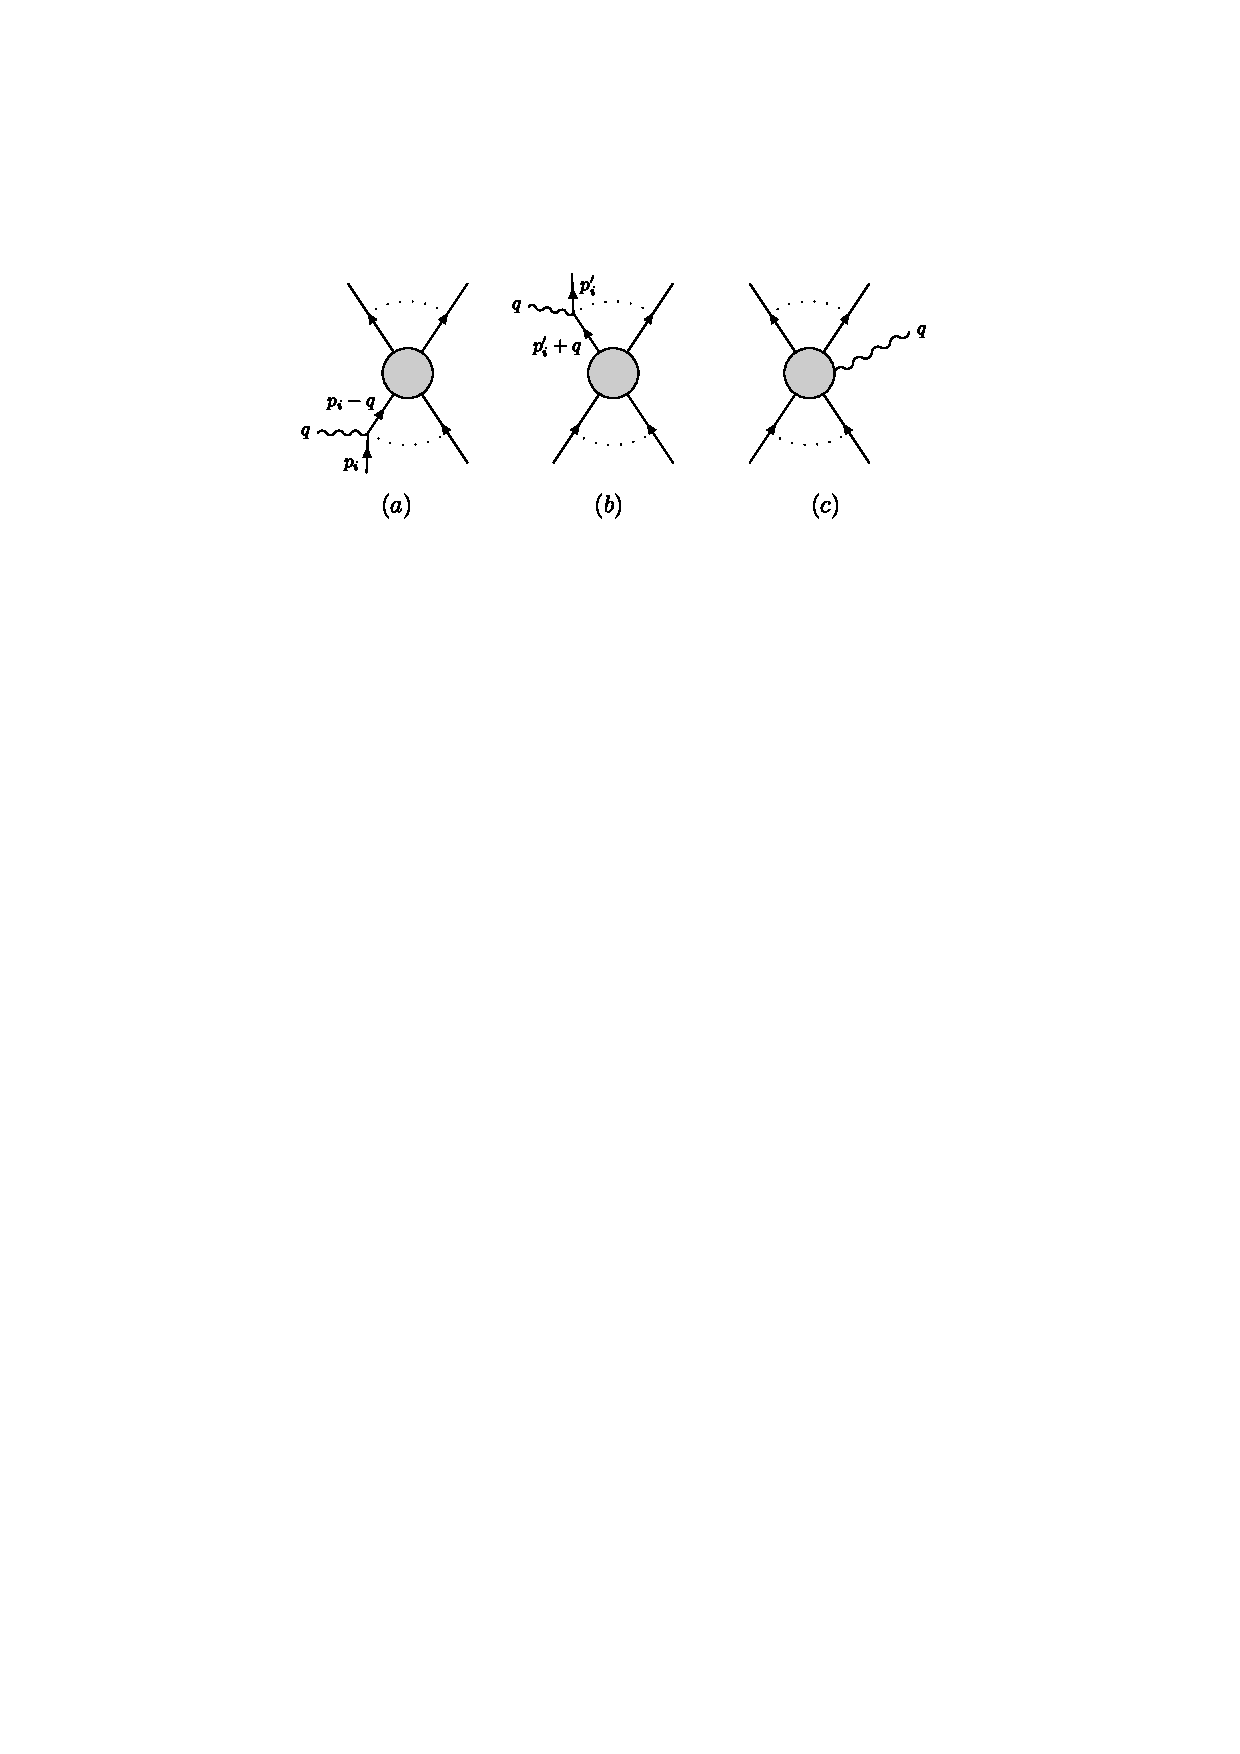
\includegraphics[width=0.8\linewidth]{figs/fig3.pdf}
	\caption{辐射软光子的三种情况}
\end{figure}
我们使用$\mathcal{A}(p,q)$表示辐射一个软光子后的振幅$\mathcal{A}(p)$表示没有辐射软光子的振幅(所有阶费曼图求和)。用$T(p_i-q)$表示原先没有辐射软光子的费曼图砍掉一个$p_i$外线但保留外线动量为非在壳的$p_i-q$得到的费曼图振幅,显然$T(p_i)u(p_i)=\mathcal{A}(p)$。

首先计算入射外线辐射软光子:
\begin{equation}
	\begin{aligned}
		Q_iT(p_i-q)\frac{(-\slashed{p}_i^\prime+\slashed{q}+m)\slashed{\epsilon}(q)}{(p_i-q)^2+m^2}u(p_i)&=-Q_iT(p_i-q)\Big[\frac{\epsilon(q)\cdot p_i+i\epsilon(q)_\mu q_\nu S^{\mu\nu}}{q\cdot p_i+\mathrm{i}0^+}\Big]u(p_i)
	\end{aligned}
\end{equation}
其中利用了$\slashed{a}\slashed{b}=-2a\cdot b-\slashed{b}\slashed{a}$,$q\cdot \epsilon_\pm(q)=0$以及狄拉克方程$(\slashed{p}+m)u(p)=0$。其中$S^{\mu\nu}=\frac{\mathrm{i}}{4}[\gamma^\mu,\gamma^\nu]$。唯一做近似的地方就是分母里面的$q^2$我们略去了,这对后面的高阶修正也不会影响。这一注意到$q=0$实际上是一个极点,这是因为在光子无线“软”的时候,多出来的那条内线传播子会无线趋于在壳,导致分母为0。

对于出射粒子辐射软光子也是类似的计算得到:
\begin{equation}\label{eq:20.17}
	\begin{aligned}
		Q^\prime_i\bar u(p_i^\prime)\frac{(-\slashed{p}_i^\prime-\slashed{q}+m)\slashed{\epsilon}(q)}{(p_i-q)^2+m^2}\bar T(p_i+q)&=Q^\prime_i\bar u(p_i^\prime)\Big[\frac{\epsilon(q)\cdot p_i+i\epsilon(q)_\mu q_\nu S^{\mu\nu}}{q\cdot p_i-\mathrm{i}0^+}\Big]\bar T(p_i-q)
	\end{aligned}
\end{equation}

至于内线发射光子,我们用$N^\mu(p,q)$表示,而且注意到$q\to0$时$N$非奇异,而且内线本身就是不在壳的,所以可以认为$N^\mu(p,q)\sim\mathcal{O}(q^0)$。三项加起来得到:
\begin{equation}\label{eq:21.3}
	\begin{aligned}
		\mathcal{A}(p,p^{\prime},q) =&\sum_\text{incoming }{ - Q _ i T ( p _ i - q )}\frac{\epsilon(q)\cdot p_i+i\epsilon(q)_{\mu}q_\nu S^{\mu\nu}}{q\cdot p_i+\mathrm{i}0^+}u(p_i)  \\
		&+\sum_{\mathrm{outgoing}}Q_{i}^{\prime}\bar{u}(p_{i}^{\prime})\frac{\epsilon(q)\cdot p_{i}^{\prime}+i\epsilon(q)_{\mu}q_{\nu}{S}^{\mu\nu}}{q\cdot p_{i}^{\prime}-\mathrm{i}0^+}\bar{T}(p_{i}^{\prime}+q)\\
		&+\epsilon(q)_{\mu}N^{\mu}(p,p^{\prime},q)
	\end{aligned}
\end{equation}
考虑最低阶修正,也就是只保留极点,得到:
\begin{equation}\label{eq:21.4}
	\boxed{
	\mathcal{A}(p,q)=\left[\sum_{i}\eta_iQ_{i}\frac{\epsilon(q)\cdot p_{i}}{q\cdot p_{i}}\right]\mathcal{A}(p)}+\mathcal{O}(1)
\end{equation}
其中对于入射粒子$\eta_i=-1$,出射粒子为$+1$。QED中辐射出光子的振幅都可以拆分成$\epsilon(q)_\mu \mathcal{M}^\mu$,振幅是相对论不变量,但是我们虽然常说$\epsilon(q)_\mu$是极化矢量,但它并不是真正意义上的矢量,因为其在lorentz变换下并不协变,而是会多出来一个正比于$q$的项\sn{我们是在Lorentz变换的意义下理解,其实矢量的这种变换完全可以理解为规范选取不同,从而从振幅的规范不变性导出结果。\cite{srednicki}}\cite{Weinberg}。为了让振幅是相对论不变量,必须有:
\begin{equation}\label{eq:21.5}
	\boxed{
	q_\mu\mathcal{M}^\mu=0}
\end{equation}
也就是Ward恒等式,也可以从Ward-高桥恒等式在U(1)对称性下导出它,实际上也就是利用电荷守恒导出它,但是前面我们的导出仅仅依赖于Lorentz不变性。现在把\ref{eq:21.4}中的$\epsilon(q)$替换为$q$我们得到:
\begin{equation}\label{eq:21.6}
	\left[\sum_i\eta_i Q_i\right]\mathcal{A}(p)=0
\end{equation}
也就是说,如果散射过程不被禁闭,也就是$\mathcal{A}(p)\neq 0$,那么这个过程必然要电荷守恒!另外说一句,我们这里的推导得到的\ref{eq:21.4}对于任意自旋的场都适用,比如对于标量QED,只需要把$S^{\mu\nu}$替换为0就好,不同的自旋对应$S^{\mu\nu}$的不同表示。

现在继续考虑两个光子的情况,两个光子由不同外线发射,在最低阶近似下只是乘上了\ref{eq:21.4}中两个因子,但是由相同外线发射就要考虑发射的先后顺序,因子形式会变化:
\begin{figure}[H]
	\centering
	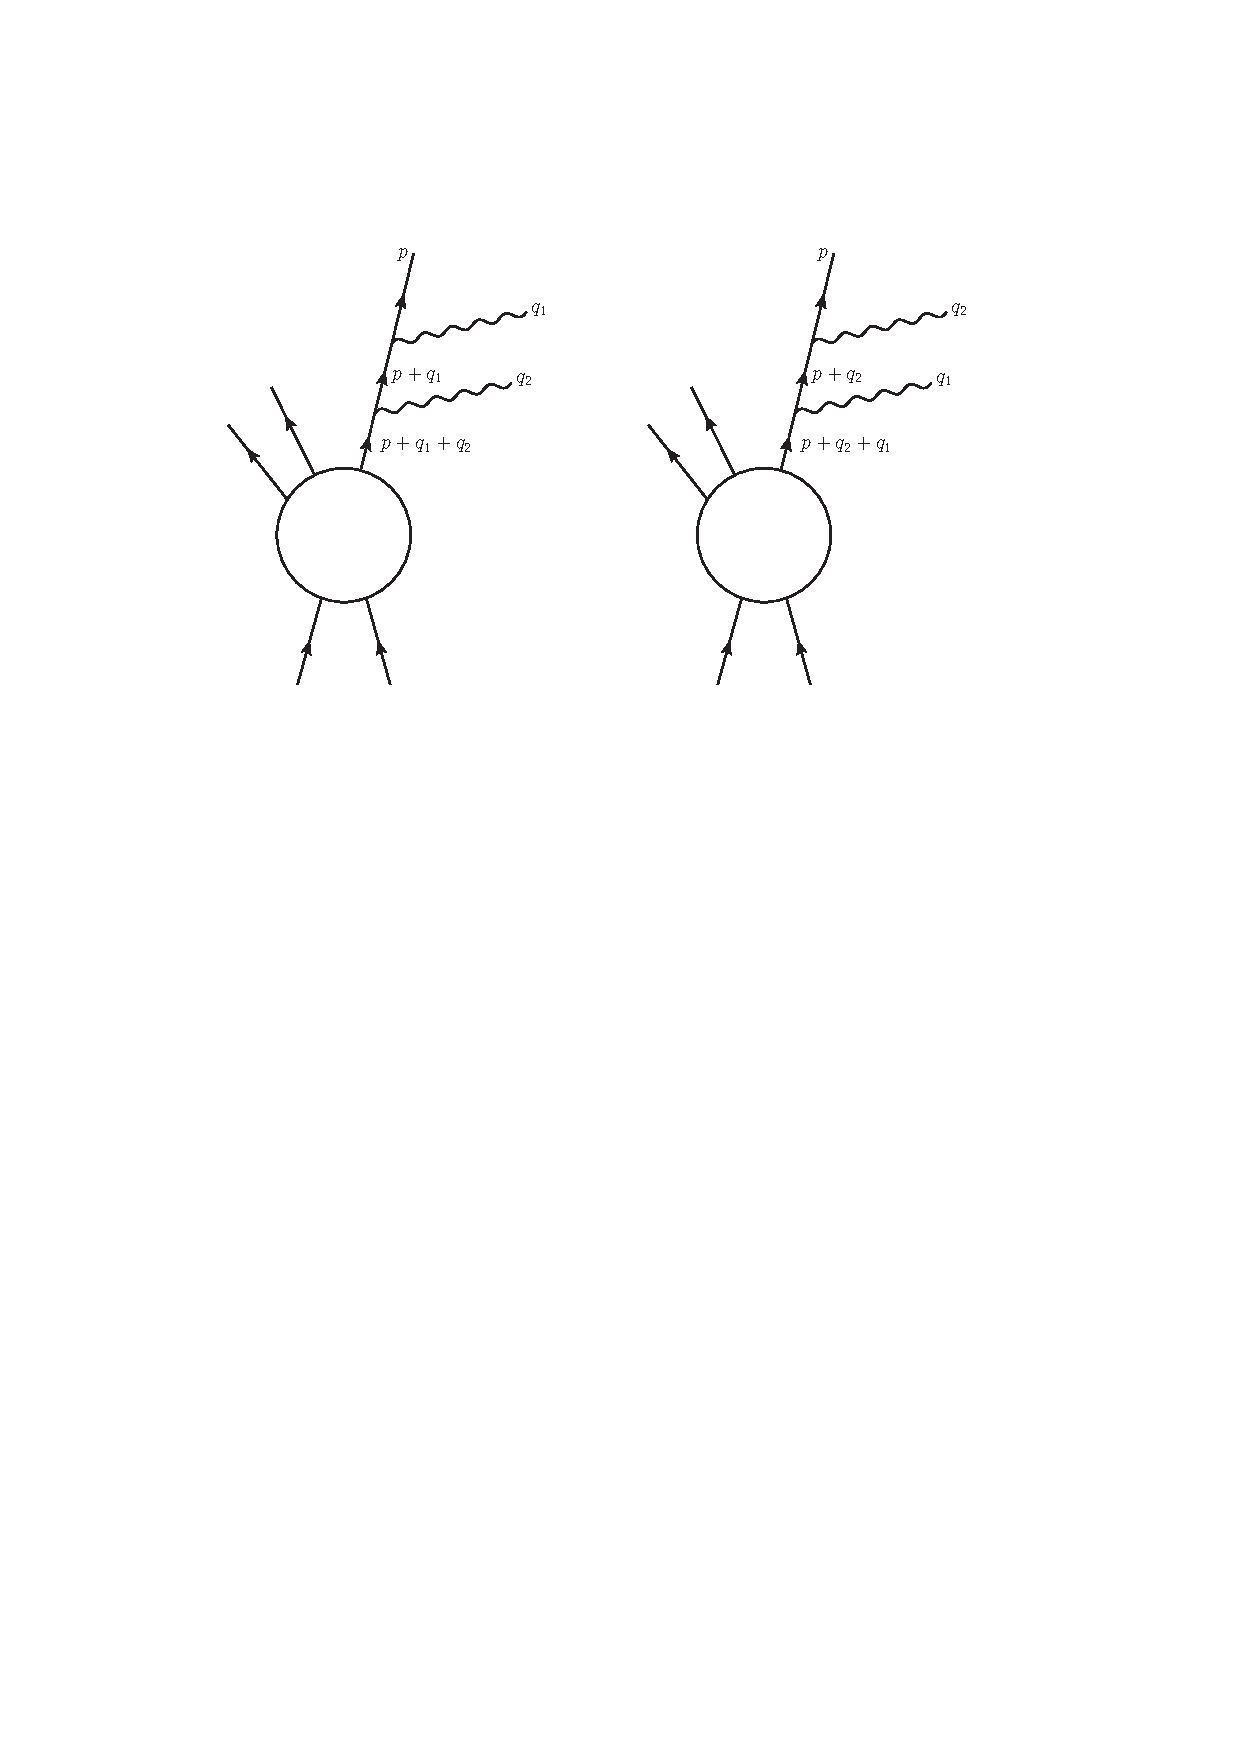
\includegraphics[width=0.8\linewidth]{figs/fig4.pdf}
	\caption{同一外线辐射两个软光子}
\end{figure}
把两幅图贡献的因子加起来得到:
\begin{equation}
	\begin{aligned}
	&\left[\frac{\eta Q\epsilon(q_1)\cdot p}{p\cdot q_1-\mathrm{i}\eta0^+}\right]\left[\frac{\eta Q\epsilon(q_2)\cdot p}{p\cdot(q_2+q_1)-\mathrm{i}\eta 0^+}\right]+\left[\frac{\eta Q\epsilon(q_2)\cdot p}{p\cdot q_2-\mathrm{i}\eta0^+}\right]\left[\frac{\eta Q\epsilon(q_1)\cdot p}{p\cdot(q_1+q_2)-\mathrm{i}\eta 0^+}\right]\\=&\left[\frac{\eta Q\epsilon(q_1)\cdot p}{p\cdot q_1-\mathrm{i}\eta0^+}\right]\left[\frac{\eta Q\epsilon(q_2)\cdot p}{p\cdot q_2-\mathrm{i}\eta 0^+}\right]	
	\end{aligned}
\end{equation}
得到的结果就是不同外腿上面的辐射两个软光子得到的因子,利用数学归纳法可以证明这一结论对于辐射任意数量的软光子都是适用的,那么最终我们只需要把因子乘起来,然后对所有外腿求和就好了,用式子表示如下:
\begin{equation}
	\boxed{\mathcal{A}(p,q_1,\ldots,q_m)=\prod_{j=1}^m\left[\sum_{i=1}^nQ_i\eta_i\frac{\epsilon(q_j)\cdot p_i}{q_j\cdot p_i}\right]\mathcal{A}(p)++\mathcal{O}(1)}
\end{equation}
前面的因子称为\textbf{eikonal因子}。推广到non-Abelian Y-M场的软定理也早有人计算过了\cite{Berends:1987me,Berends:1988zn,Mangano:1987kp,Mangano:1990by},软定理更多更一般的推广见\cite{McLoughlin:2022ljp}的文献索引。

现在来考虑辐射一个软引力子的情况,考虑第一节引入的标量场模型,传播子为:
\begin{equation}
	-\frac{i }{(p+\eta q)^2+m^2}
\end{equation}
顶点由\ref{eq:20.17}给出,但是由于\ref{eq:20.10},要与$\epsilon^{\mu\nu}$缩并,正比于$\eta_{\mu\nu}$的项没有贡献。以出射外线辐射软引力子为例,给出因子:
\begin{equation}
	i\sqrt{32\pi G}\varepsilon^{\mu\nu}p_{\mu}p_{\nu}\frac{-i}{\left(p+q\right)^{2}+m^{2}}\rightarrow\sqrt{8\pi G}\frac{\varepsilon^{\mu\nu}p_{\mu}p_{\nu}}{p\cdot q}
\end{equation}
求和后得到:
\begin{equation}
	\boxed{
	\mathcal{A}(p,q)=\left[\sum_i\frac{\kappa_i}{2}\eta_i\frac{\epsilon_{\mu\nu}(q)p_i^\mu p_i^\nu}{q\cdot p_i}\right]\mathcal{A}(p)+\mathcal{O}(1)}
\end{equation}

引力子同样有类似于\ref{eq:21.5}的恒等式,由此我们可以得到所有的$\kappa_i$都是相等的\sn{这里有点循环论证了,因为前面为了推导的方便我们同一取$\kappa_i=\sqrt{32\pi G}$},也就是等效原理!而自旋大于二的软粒子的软定理沿用上面的方法给出的限制就太强了,以至于散射$\mathcal{S}$矩阵必须trivial,所以一般认为自旋大于二的无质量粒子在“变软”的时候就脱耦合了。
\section{Subleading and subsubleading order soft theorem}
考虑动量为$\delta q,\delta \to0$的软光子辐射,$\pm$表示软光子的螺旋度,而$\ell_i$表示其它粒子的螺旋度,则更一般的软定理可以用洛朗展开写成:
\begin{equation}
	\mathcal{A}_{\ell_1,...,\ell_n,\pm}(p,\delta q)=\left[\sum_{a=0}^\infty\delta^{-1+a}S_\pm^{(a)}\right]\mathcal{A}_{\ell_1,...,\ell_n}(p)
\end{equation}
次领头阶的计算可以从\ref{eq:21.5}式出发,将\ref{eq:21.3}中所有的$\epsilon$替换为动量,保留到$\mathcal{O}(\delta^0)$,并且令等式左边为0。注意到这一阶近似下可以有$N^\mu(p,q)\approx N^\mu(p,0)$,得到:
\begin{equation}
	-q^{\mu}N_{\mu}(p,0)=\cancelto{0}{\frac{1}{\delta}\sum_{i=1}^{n}\eta_{i}Q_{i}\mathcal{A}(p)}+q^{\mu}\sum_{i=1}^{n}Q_{i}\frac{\partial}{\partial p_{i}^{\mu}}\mathcal{A}(p)
\end{equation}
其中第一项为0是因为电荷守恒\ref{eq:21.6},第二项中的$\partial_{p_i}$只作用于$\mathcal{A}$中的$T$,不作用于$u$\sn{因为这个式子的导出,是对$T(p\pm q)$展开得到的。}。这样就确定出了$N^\mu$\sn{其实只能确定到某个与$q$无关的矢量$v$,满足$q\cdot v=0$,但是这样的$v$实际上不存在。},再带回到\ref{eq:21.3}得到:
\begin{equation}
	A^\mu=\sum_{i=1}^nQ_i\left[\frac{\eta_ip_i^\mu}{\delta q\cdot p_i}+\frac{q^\nu p_i^\mu}{q\cdot p_i}\frac{\partial}{\partial p_i^\nu}-\frac{iq_\nu S_i^{\mu\nu}}{q\cdot p_i}-\frac{\partial}{\partial p_{i\mu}}\right]\mathcal{A}(p)+\mathcal{O}(\delta)
\end{equation}
这个式子里面的$\partial_{p_i}$就是作用于整个$\mathcal{A}$了。定义:
\begin{equation}
	L_i^{\mu\nu}=i\left(p_i^\mu\frac{\partial}{\partial p_{i\nu}}-p_i^\nu\frac{\partial}{\partial p_{i\mu}}\right),\quad J^{\mu\nu}_i+S_i^{\mu\nu}
\end{equation}
这里$S_i^{\mu\nu}$要根据第i个粒子的自旋去选取对应的Lorentz群不可约表示,比如$s=0,S^{\mu\nu}=0;s=\frac{1}{2},S^{\mu\nu}=\frac{i}{4}[\gamma^\mu,\gamma^\nu]$。这样我们就得到了包含subleading修正的软定理(LBK定理\cite{PhysRevLett.20.86,PhysRev.110.974}):
\begin{equation}
	\begin{aligned}S_{\pm}^{(0)}&=\sum_{i=1}^nQ_i\eta_i\frac{\epsilon_{\pm\mu}(q)p_i^\mu}{q\cdot p_i},\quad\text{and}\quad S_{\pm}^{(1)}&=-i\sum_{i=1}^nQ_i\frac{\epsilon_{\pm\mu}(q)q_\nu J_i^{\mu\nu}}{q\cdot p_i}\end{aligned}
\end{equation}
同样的方法可以推导出软引力子定理的subleading和subsubleading的修正项\sn{软定理已经使用不同的方法推了很多遍,文献\cite{McLoughlin:2022ljp,Brandhuber:2022qbk}中有不同证明方法的文献索引,而且还有对于更复杂的非阿贝尔规范理论的软定理讨论。}\cite{PhysRevD.90.084035,PhysRev.168.1623,White:2014qia,Broedel:2014fsa}:
\begin{equation}
	\begin{gathered}
		S_{\pm}^{(0)}=\frac{\kappa}{2}\sum_{i=1}^{n}\eta_{i}\frac{\epsilon_{\pm\mu\nu}(q)p_{i}^{\mu}p_{i}^{\nu}}{q\cdot p_{i}},\quad S_{\pm}^{(1)}=-i\frac{\kappa}{2}\sum_{i=1}^{n}\frac{\epsilon_{\pm\mu\nu}(q)p_{i}^{\mu}q_{\lambda}J_{i}^{\nu\lambda}}{q\cdot p_{i}}, \\
		S_{\pm}^{(2)}=-\frac{\kappa}{4}\sum_{i=1}^{n}\eta_{i}\frac{\epsilon_{\pm\mu\nu}(q)q_{\rho}q_{\sigma}J_{i}^{\mu\rho}J_{i}^{\nu\sigma}}{q\cdot p_{i}}
	\end{gathered}
\end{equation}

\section{Massless QED}
本章用天球的视角来看QED理论,为下一节做准备,本节的讨论都局限于比较简单的,不含磁荷而且电子没有质量的QED理论,但是基于此推出的许多结论实际上是普适的,可以推广到有质量QED上\cite{Strominger:2017zoo}。
\subsection{Classical}
弯曲时空中QED作用量:
\begin{equation}
	S_{EM}=-\frac{1}{2e^2}\int{F}\wedge\star F +S_M=-\frac{1}{4e^2}\int \mathrm{d}^4x\sqrt{-g}F_{\mu]nu}F^{\mu\nu}+S_M
\end{equation}
其中$S_M$由$j^\nu A_\nu$形式给出相互作用项,即$j^\nu=-\frac{\delta S_M}{\delta A^\nu}$。Maxwell场方程有下面简洁形式:
\begin{equation}
	\begin{cases}
		dF=0&\Rightarrow \nabla_\mu F_{\nu\rho}+\nabla_\nu F_{\rho\mu}+\nabla_\rho F_{\mu\nu}=0\\
		d\star F=e^2\star j&\Rightarrow \nabla_\mu F_{\mu\nu}=e^2j_\nu
	\end{cases}
\end{equation}
下式给出了整个空间内的净电荷/磁荷\sn{后文$\star,*$指的都是Hodge dual}:
\begin{equation}
	Q_E=\frac{1}{e^2}\int_{\mathcal{S}^2_\infty}\star F=\int_{\Sigma}\star j,\quad Q_M=\frac{1}{2\pi}\int_{\mathcal{S}^2_\infty} F
\end{equation}
它们是量子化的,只能取整数。QED是$U(1)$规范理论,在$A\mapsto A+d\varepsilon$的规范变换下理论不变,后文不加说明都在所谓\textbf{retarded radial 规范}下进行计算\cite{He:2014cra,Kapec:2015ena}:
\begin{equation}
	\begin{aligned}
		&\mathcal{I}^+: A_r=0,\quad A_u|_{\mathcal{I}^+}=0\\
		&\mathcal{I}^-: A_r=0,\quad A_v|_{\mathcal{I}^-}=0
	\end{aligned}
\end{equation}
在$\mathcal{I}^{\pm}$附近可以把$A,F$展开成$\mathcal{O}(1/r)$的形式,用$A^{(i)},F^{(i)}$表示$r^{-i}$项前的系数,那么在这一规范下有\sn{各项系数都只和$(u,z,\bar z)$相关了}:
\begin{equation}
	F_{ur}^{(0)}=A_u^{(0)}, F_{z\bar z}^{(0)}=\partial_z A_{\bar z}^{(0)}-\partial_{\bar z}A_z^{(0)},F_{uz}^{(0)}=\partial_u A_z^{(0)},F_{rz}^{(0)}=-A_z^{(1)}
\end{equation}
而且我们所关心的场位形在$\mathcal{I}^{+}_{+}$处为真空,即满足:
\begin{equation}
	\left.F_{ur}\right|_{\mathcal{I}_{+}^{+}}=\left.F_{uz}\right|_{\mathcal{I}_{+}^{+}}=0
\end{equation}
$\mathcal{I}^-$处类似。但这个规范选取就如库伦规范$\nabla\cdot \mathbf{A}=0$一样没有完全确定规范,$A^{(0)}_z$还可以进行下面的所谓Large gauge transformation:
\begin{equation}
	A^{(0)}_z\mapsto A^{(0)}_z+\partial_z\varepsilon(z,\bar z),\quad \forall \varepsilon\in C^\infty\left[C\mathcal{S}^2\right]
\end{equation}
规范变换是一种冗余,但是这里的Large gauge transformations 最大的特点就是在无穷远处不归零,这导致很多时候分部积分的边界项不能丢去,确确实实的成为了一个对称性,后面马上会看到会对应无穷多个守恒荷。

运动电荷激发的电磁场即所谓Li\'enard\mbox{-}Wiecher势\cite{Jackson1998ClassicalE3}。这里我们在天球坐标下将advanced和retarded势统一写为:
\begin{equation}
	F_{rt}(\vec{x},t)=\frac{e^2}{4\pi}\sum_{k=1}^n\frac{Q_k\gamma_k\left(r-t\hat{x}\cdot\vec{\beta}_k\right)}{\left|\gamma_k^2\left(t-r\hat{x}\cdot\vec{\beta}_k\right)^2-t^2+r^2\right|^{3/2}},\quad r^2=\vec{x}\cdot\vec{x},\quad\vec{x}=r\hat{x}
\end{equation}
其中我们假设所有电荷之间匀速运动,而且相互作用可忽略,这个假设有点强,但是请\textbf{相信}后面导出的结论是可以推广到一般情形的。现在计算在天球上的极限:
\begin{equation}
	\begin{aligned}
		&\left.F_{rt}\right|_{\mathcal{I}^{+}}=\frac{e^{2}}{4\pi r^{2}}\sum_{k=1}^{n}\frac{Q_{k}}{\gamma_{k}^{2}(1-\hat{x}\cdot\vec{\beta}_{k})^{2}}\\
		&\left.F_{rt}\right|_{\mathcal{I}^{-}}=\frac{e^{2}}{4\pi r^{2}}\sum_{k=1}^{n}\frac{Q_{k}}{\gamma_{k}^{2}(1+\hat{x}\cdot\vec{\beta_{k}})^{2}}
	\end{aligned}
\end{equation}
取极限,得到:
\begin{equation}
	\boxed{
	\left.F_{rt}\right|_{\mathcal{I}^{+}_-}\neq \left.F_{rt}\right|_{\mathcal{I}^{-}_+}}
\end{equation}
正是这个式子说明了要严格区分$\mathcal{I}^{+}_-,\mathcal{I}^{-}_{+}$和$i^0$。但是,因为$F_{ru}=F_{rt}=F_{rv}$:
\begin{equation}
	\boxed{
		\lim\limits_{r\to\infty}r^2F_{ru}(\hat{x})\Big|_{\mathcal{I}_{-}^+}=\lim\limits_{r\to\infty}r^2F_{rv}(-\hat{x})\Big|_{\mathcal{I}_{+}^-}
	}
\end{equation}
也就是说场在两个天球上是对径认同的,这也是为什么前面$\mathcal{I}^{\pm}$天球的角向选取是antipodal的,上边的式子可以写成下面很简洁的形式:
\begin{equation}
	\boxed{
	\left.F_{ru}^{(2)}(z,\bar z)\right|_{\mathcal{I}^{+}_-}=\left.F_{rv}^{(2)}(z,\bar z)\right|_{\mathcal{I}^{-}_+}
	}
\end{equation}
这个式子是普适的,而且非常重要,是后面散射问题的核心。现在考虑任意一个天球上的对径认同的函数:
\begin{equation}
	\varepsilon(z,\overline{z})|_{\mathcal{I}_{-}^{+}}=\varepsilon(z,\overline{z})|_{\mathcal{I}_{+}^{-}}
\end{equation}
定义下面的future charges和past charges:
\begin{equation}
	\boxed{
		Q_{\varepsilon}^{+}=\frac{1}{e^{2}}\int_{\mathcal I_{-}^{+}}\varepsilon*F,\quad Q_{\varepsilon}^{-}=\frac{1}{e^{2}}\int_{\mathcal I_{+}^{-}}\varepsilon*F
	}
\end{equation}
由于Hodge对偶后出来的体积元$\propto r^2$,所以在天球上$r\to\infty$,$F\to F^{(2)}$,再根据对径认同的条件,这样对于任意一个函数$\varepsilon$,我们都给出了一个“电荷”守恒律:
\begin{equation}
	\boxed{
	Q_\varepsilon^+=Q_\varepsilon^-
	}
\end{equation}
对于$\varepsilon$是常函数情形,就得到了一般的电荷守恒律。利用Stokes公式\sn{$\int_{\partial \Omega}\omega =\int_{ \Omega}d\omega$}可以改写$Q_\varepsilon^{\pm}$为\sn{$Q_\varepsilon^-$只用把$+\mapsto -$}:
\begin{equation}
	Q_\varepsilon^+=\frac{1}{e^2}\int_{\mathcal{I}^+}\mathrm{d}\varepsilon\wedge*F+\int_{\mathcal{I}^+}\varepsilon*j+\cancelto{0}{\frac{1}{e^2}\int_{\mathcal{I}_+^+}\varepsilon*F}
\end{equation}
最后一项为0是因为我们假设电子是无质量的,这样电子就是从$\mathcal{I}^-\to\mathcal{I}^+$,而不是$i^{-}\to i^+$,所以$F|_{\mathcal{I}_+^{+}}=0$。第一项是Soft term $Q_S^+$与软光子的产生湮灭有关,第二项由于是与流耦合,所以叫Hard term $Q_H^+$与带电实物粒子有关。将上面的微分形式写成分量形式\sn{其中使用了Bianchi恒等式:$\partial_{u}F_{ru}^{(2)}+D^{z}F_{uz}^{(0)}+D^{\bar{z}}F_{u\bar{z}}^{(0)}+e^2j_{u}^{(2)}=0$}:
\begin{equation}
	Q_{\varepsilon}^{+}=\underbrace{-\frac{1}{e^{2}}\int_{\mathcal{I}^{+}}dud^{2}z\left(\partial_{z}\varepsilon F_{u\bar{z}}^{(0)}+\partial_{\bar{z}}\varepsilon F_{uz}^{(0)}\right)}_{Q_{S}^{+}}+\underbrace{\int_{\mathcal{I}^{+}}dud^{2}z\varepsilon\gamma_{z\bar{z}}j_{u}^{(2)}}_{Q_{H}^{+}}
\end{equation}
定义Soft photon mode $N_z$:
\begin{equation}\label{eq:23.18}
	N_{z}\equiv \int_{-\infty}^{\infty}duF_{uz}^{(0)}=\lim_{\omega\to0}\int_{-\infty}^{\infty}duF_{uz}^{(0)}e^{i\omega u}
\end{equation}
再次看到$N_z$对应的是电磁场的零频部分,也就是软光子部分,而且有:
\begin{equation}
	\begin{aligned}
		\partial_{\bar{z}}N_{z}-\partial_{z}N_{\bar{z}}& =\int_{-\infty}^{\infty}du\left[\partial_{\bar{z}}F_{uz}^{(0)}-\partial_{z}F_{u\bar{z}}^{(0)}\right]  \\
		&=-\int_{-\infty}^{\infty}du\left.\partial_{u}F_{z\bar{z}}^{(0)}=-F_{z\bar{z}}^{(0)}\right|_{\mathcal{I}_{-}^{+}}^{\mathcal{I}_{+}^{+}}=0
	\end{aligned}
\end{equation}
最后等于0是因为$F_{z\bar z}|_{\mathcal{I}_{+}^{\pm}}=0$,本质上是因为没有磁单极子,磁场不是long-range的,在无穷远处为0\sn{因为$F_{z\bar z}=\frac{\partial x^{\mu}}{\partial z}\frac{\partial x^{\nu}}{\partial\bar{z}}F_{\mu\nu}=\frac{\partial x^{i}}{\partial z}\frac{\partial x^{j}}{\partial\bar{z}}F_{ij}$,而规范场强的空间分量$F_{ij}$只和磁场有关。}。所以$N_z$无旋,可以由此引申出一个实标量场$N$作为其原函数:
\begin{equation}
	N_z\equiv e^2\partial_zN=\int_{-\infty}^{\infty}duF_{uz}^{(0)}=A_{z}^{(0)}|_{\mathcal{I}_{+}^{+}}-A_{z}^{(0)}|_{\mathcal{I}_{-}^{+}}
\end{equation}
利用$N$,future charges可以写成下面简洁形式:
\begin{equation}\label{eq:23.21}
	Q_{\varepsilon}^{+}=2\int_{\mathcal{S}_\infty^2} d^{2}zN\partial_{z}\partial_{\bar{z}}\varepsilon+\int_{\mathcal I^{+}}dud^{2}z\varepsilon\gamma_{z\bar{z}}j_{u}^{(2)}
\end{equation}
对past charge也可以来上面的这一套:
\begin{equation}\label{eq:23.21.2}
	Q_{\varepsilon}^{-}=-2\int_{\mathcal{S}_\infty^2} d^{2}zN^-\partial_{z}\partial_{\bar{z}}\varepsilon+\int_{\mathcal I^{-}}dvd^{2}z\varepsilon\gamma_{z\bar{z}}j_{v}^{(2)}
\end{equation}
\subsection{Quantization}
上面讨论的都是经典场,现在进行量子化,目的是说明前面定义的future charge 和 past charges 都是 Large gauge transformations 对应的生成元算符。量子化方案选用正则量子化方案,这里使用的方法不需要事先对时空进行3+1分解,是协变的方法\cite{Ashtekar1987AsymptoticQ,Frolov:1979ab,1989thyg.book.....H,Lee:1990nz,Wald:1999wa}。

经典力学的正则形式是建立在辛几何上的,也就是给相流形上配备了一个非退化的、闭的二形式\cite{Arnold}:
\begin{equation}\label{eq:23.22}
	\Omega=\frac{1}{2}\omega_{IJ}dx^I\wedge dx^J
\end{equation}
而且可以证明,可以通过选取不同的广义坐标局部的将$\omega_{IJ}$化为下面的矩阵:
\begin{equation}
	\omega_{IJ}=\left.\left[\begin{matrix}0&1_{N\times N}\\-1_{N\times N}&0\end{matrix}\right.\right]
\end{equation}
力学量的Possion括号由下式给定:
\begin{equation}
	\{A,B\}=\Omega^{IJ}\partial_IA\partial_JB
\end{equation}
相空间是运动方程的解,可以与初始值一一对应。

到了场论这边,相空间我们可以选取为某一个柯西面$\Sigma$上的场位形。场$\phi$本身是流形上的微分形式,\ref{eq:21.22}中的$dx$应该替换为$\delta\phi$,这里$\delta$是场位形的在壳变分,也就是说$\phi+\delta \phi$仍然是场方程的解。场本身是定义在某个纤维丛上的,可以粗浅的理解为两个流形拼起来,而$d$是底流形上的微分形式算子,$\delta$事实上是另一个正交的微分形式算子,所以$\delta\phi$在$\delta$的意义上是1\mbox{-}form,在$d$的意义上$\delta$的作用不会改变其是几形式,这样$\Omega$形如$\delta\phi\wedge\delta\varphi$从$\delta$的意义上看就是个二形式。构建的微分形式还应当满足规范不变性,闭且非退化,而且还要对柯西面的不同选取一致,利用\cite{Wald:1999wa}中方法可以得到$U(1)$规范场的辛形式为:
\begin{equation}
	\Omega_{\Sigma}=-\frac{1}{e^{2}}\int_{\Sigma}\delta(*F)\wedge\delta A
\end{equation}
将柯西面选取为$\mathcal{I}^{\pm}$,得到分量为:
\begin{equation}
	\begin{aligned}
		\omega_{uz\bar{z}}|_{\mathcal{I}}+& =-\frac{1}{e^{2}}\left[\delta(*F)_{uz}\wedge\delta A_{\bar{z}}+\delta(*F)_{\bar{z}u}\wedge\delta A_{z}+\delta(*F)_{z\bar{z}}\wedge\delta A_{u}\right]_{\mathcal{I}^{+}}  \\
		&=-\frac{i}{e^{2}}\left[\delta F_{uz}^{(0)}\wedge\delta A_{\bar{z}}^{(0)}+\delta F_{u\bar{z}}^{(0)}\wedge\delta A_{z}^{(0)}\right],
	\end{aligned}
\end{equation}
其中利用了:\sn{注意到Levi-Civita符号不是张量,而是张量密度,$\sqrt{-g}\epsilon$才是张量,然后利用Hodge dual定义爆算即可}
\begin{equation}
	(*F)_{uz}=i\left(F_{uz}-F_{rz}\right),\quad(*F)_{z\bar{z}}=ir^{2}\gamma_{z\bar{z}}F_{ru}
\end{equation}
最终得到辛形式:
\begin{equation}\label{eq:23.29}
	\Omega_{\mathcal{I}^+}=\frac{1}{e^2}\int dud^2z\left[\delta F_{uz}^{(0)}\wedge\delta A_{\bar{z}}^{(0)}+\delta F_{u\bar{z}}^{(0)}\wedge\delta A_{z}^{(0)}\right]
\end{equation}
总是可以把$A_z$的$u\to\pm {\infty}$,也就是$\mathcal{I}^+_{\pm}$的与$u$无关的部分分离出去,这一部分又总是可以写成某个天球上标量场的导数,因为要求$F_{z\bar z}|_{\mathcal{I}_{+}^{\pm}}=0$:
\begin{equation}
	A_z^{(0)}(u,z,\bar{z})=\hat{A}_z(u,z,\bar{z})+\partial_z\phi(z,\bar{z}),\quad\partial_z\phi\equiv\frac{1}{2}\left[\left.A_z^{(0)}\right|_{\mathcal I_+^+}+\left.A_z^{(0)}\right|_{\mathcal I_-^+}\right]
\end{equation}
利用上面的分解以及soft photon mode重写\ref{eq:23.29}:
\begin{equation}
	\Omega_{\mathcal{I}^{+}}=\frac{2}{e^{2}}\int dud^{2}z\partial_{u}\delta\hat{A}_{z}\wedge\delta\hat{A}_{\bar{z}}-2\int d^{2}z\partial_{z}\delta\phi\wedge\partial_{\bar{z}}\delta N
\end{equation}
现在考虑正则量子化,场变成算符,而Poisson括号换成Dirac括号:\sn{$\{\quad,\quad\}\mapsto\frac{1}{i}[\quad,\quad]$}
\begin{equation}
	\begin{aligned}-\frac{2}{e^2}\left[\partial_u\hat A_z(u,z,\bar z),\hat A_{\bar w}(u',w,\bar w)\right]&=i\delta(u-u')\delta^2(z-w),\\2\left[\partial_z\phi(z,\bar z),\partial_{\bar w}N(w,\bar w)\right]&=i\delta^2(z-w).\end{aligned}
\end{equation}
积分得到:\sn{这里$$\Theta(u)=\frac{1}{\pi i}\int\frac{d\omega}{\omega}e^{i\omega u}=\begin{cases}+1&,u>0\\-1&,u<0\end{cases}$$}
\begin{equation}
	\begin{aligned}
		\left[\hat{A}_{z}(u,z,\bar{z}),\hat{A}_{\bar{w}}(u^{\prime},w,\bar{w})\right]& =-\frac{ie^{2}}{4}\Theta(u-u^{\prime})\delta^{2}(z-w),  \\
		[\phi(z,\bar{z}),N(w,\bar{w})]& =-\frac{i}{4\pi}\log|z-w|^{2}+f(z,\bar{z})+g(w,\bar{w}). 
	\end{aligned}
\end{equation}

\subsection{Large guage symmetry}
利用上面发展的对易式可以去计算$Q_\varepsilon^{\pm}$与场算符的对易关系,注意到物质场部分$Q_H$始终和规范场$A$对易,所以:
\begin{equation}
	\begin{aligned}&\left[Q_{\varepsilon}^{+},A_{z}^{(0)}(u,z,\bar{z})\right]=i\partial_{z}\varepsilon(z,\bar{z}),\\&\left[Q_{\varepsilon}^{-},A_{z}^{(0)}(v,z,\bar{z})\right]=i\partial_{z}\varepsilon(z,\bar{z}).\end{aligned}
\end{equation}
所以前面定义的守恒荷其实就是对径认同的Large gauge transformation的生成元,自然就是一个守恒荷!前面的讨论一直忽略了流耦合项$S_M$,加入后对前面的结论不会有影响,注意到$Q_S$与物质场对易,根据Noether定理:
\begin{equation}
	\left[j_{u}^{(2)}(u',w,\bar{w}),\Phi_{k}(u,z,\bar{z})\right]=-Q_{k}\Phi_{k}(u,z,\bar{z})\gamma^{z\bar{z}}\delta^{2}(z-w)\delta(u-u')
\end{equation}
这意味着:
\begin{equation}\label{23.36}
	\left[Q_\varepsilon^+,\Phi_k(u,z,\bar{z})\right]=\left[\int_{\mathcal{I}^+}\varepsilon*j,\Phi_k(u,z,\bar{z})\right]=-Q_k\varepsilon(z,\bar{z})\Phi_k(u,z,\bar{z})\equiv i\delta_\varepsilon\Phi_k(u,z,\bar{z})
\end{equation}
所以$Q_S$生成规范场的规范变换,$Q_H$生成费米场规范变换,合起来$Q_\varepsilon$生成$\mathcal{I}^+$上的local规范变换。
\section{Ward indentity = Soft theorem}
\subsection{Ward indentity of $\mathcal{S}$\mbox{-}Matrix}
量子力学里面就知道守恒意味着与哈密顿量对易,而$\mathcal{S}\sim \exp{iHT}$,所以前面的守恒荷会和$\mathcal{S}$对易:\sn{初末态基底选取平面波。}
\begin{equation}\label{eq:24.1}
	\boxed{\langle\mathrm{out}|\left(Q_\varepsilon^+\mathcal{S}-\mathcal{S}Q_\varepsilon^-\right)|\mathrm{in}\rangle=0}
\end{equation}
这样一个简单的式子就是$\mathcal{S}$\mbox{-}Matrix的Ward identity。利用\ref{eq:23.21}和\ref{eq:23.21.2}得到:
\begin{equation}
	\begin{aligned}
		Q_\varepsilon^-|\mathrm{in}\rangle&=-2\int d^2z\partial_{\bar{z}}\varepsilon\partial_zN^-(z,\bar{z})|\mathrm{in}\rangle+\sum_{k=1}^mQ_k^\mathrm{in}\varepsilon(z_k^\mathrm{in},\bar{z}_k^\mathrm{in})|\mathrm{in}\rangle \\
		\langle\mathrm{out}|Q_\varepsilon^+&=2\int d^2z\partial_z\partial_{\bar{z}}\varepsilon\langle\mathrm{out}|N(z,\bar{z})+\sum_{k=1}^nQ_k^\mathrm{out}\varepsilon(z_k^\mathrm{out},\bar{z}_k^\mathrm{out})\langle\mathrm{out}|
	\end{aligned}
\end{equation}
第一项没啥好说的,后面会讨论其物理含义,第二项的计算稍微提一下。首先我们假设入射态是$m$个hard particles,而且来自于天球上的点$z_k^{\mathrm{in}}$,\ref{23.36}给出了守恒荷与物质场之间的对易关系,实际上,不难证明守恒荷和产生湮灭算符也满足同样的对易关系\sn{比如标量场\cite{srednicki}$$a^{\dagger}(\mathbf{k})=-i\int d^{3}xe^{ikx}\stackrel{\leftrightarrow}{\partial_{0}}\varphi(x)$$}。以两个入射粒子为例:
\begin{equation}
	\begin{aligned}
		Q^-_{\varepsilon}\ket{\text{in}}&\sim Q^-_{\varepsilon}a_1^\dagger a_2^\dagger\ket{0}\\
		&\sim \left[Q^-_{\varepsilon},a_1^\dagger a_2^\dagger\right]\ket{0}+\cancelto{0}{a_1^\dagger a_2^\dagger Q^-_{\varepsilon}\ket{0}}\\
		&\sim  \left[Q^-_{\varepsilon},a_1^\dagger \right]a_2^\dagger\ket{0}+a_1^\dagger\left[Q^-_{\varepsilon},a_2^\dagger \right]\ket{0}\\
		&\sim Q_1\varepsilon_1\ket{\text{in}}+Q_2\varepsilon_2\ket{\text{in}}
	\end{aligned}
\end{equation}
第二行我们利用了真空态一定是没荷的。现在可以把\ref{eq:24.1}写为:
\begin{equation}
	\begin{aligned}
		2\int d^2z\partial_z\partial_{\bar{z}}\varepsilon\langle\text{out}|&\left(N(z,\bar{z})\mathcal{S}-\mathcal{S}N^-(z,\bar{z})\right)|\text{in}\rangle\\&=\left[\sum_{k=1}^mQ_k^\text{in}\varepsilon(z_k^\text{in},\bar{z}_k^\text{in})-\sum_{k=1}^nQ_k^\text{out}\varepsilon(z_k^\text{out},{\bar{z}}_k^\text{out})\right]\langle\text{out}|\mathcal{S}|\text{in}\rangle
	\end{aligned}
\end{equation}
取$\varepsilon(z,\bar z)=\frac{1}{w-z}$,则上式可以写为如下形式:\sn{$$\partial_{\bar{z}}\frac{1}{z-w}=2\pi\delta^2(z-w)$$}
\begin{equation}\label{eq:24.5}
	4\pi\langle\mathrm{out}|\left(\partial_zN\mathcal{S}-\mathcal{S}\partial_zN^-\right)|\mathrm{in}\rangle=\left[\sum_{k=1}^m\frac{Q_k^\mathrm{in}}{z-z_k^\mathrm{in}}-\sum_{k=1}^n\frac{Q_k^\mathrm{out}}{z-z_k^\mathrm{out}}\right]\langle\mathrm{out}|\mathcal{S}|\mathrm{in}\rangle 
\end{equation}
这个等式其实就是带有U(1) K$\breve{\text{a}}$c-Moody current的$\text{CFT}_2$的Ward恒等式\cite{Blumenhagen:2009zz,He:2015zea,Strominger:2013lka,Nande:2017dba}。
\subsection{Mode expansion}
本部分的终极目标是证明Ward恒等式可以联系渐近对称性和软定理,前文从相空间角度给出了Ward恒等式,在动量空间给出了软定理,是时候在动量空间重写Ward恒等式了,重点就是将场算符用平面波展开,也就是正则量子化的过程。free mode expansion 弯曲时空量子力学领域已经不少人算过了,U(1)规范理论结果如下:
\begin{equation}
	A_{\nu}(x)=e\sum_{\alpha=\pm}\int\frac{d^3q}{\left(2\pi\right)^3}\frac{1}{2\omega_q}\left[\varepsilon_{\nu}^{*\alpha}(\vec{q})a_{\alpha}^{\mathrm{out}}(\vec{q})e^{iq\cdot x}+\varepsilon_{\nu}^{\alpha}(\vec{q})a_{\alpha}^{\mathrm{out}}(\vec{q})^\dagger e^{-iq\cdot x}\right]
\end{equation}
$q$是平面波在壳动量$q^2=0$,$\varepsilon^\pm_\mu$是极化矢量,常常取为:
\begin{equation}\label{eq:24.7}
	\varepsilon^{+\mu}(\vec{q})=\frac1{\sqrt{2}}\left(\bar{z},1,-i,-\bar{z}\right),\quad\varepsilon^{-\mu}(\vec{q})=\frac1{\sqrt{2}}\left(z,1,i,-z\right),\quad q_{\mu}\varepsilon^{\pm\mu}(\vec{q})=0,\quad\varepsilon_{\alpha}^{\mu}\varepsilon_{\beta\mu}^{*}=\delta_{\alpha\beta}
\end{equation}
产生湮灭算符之间满足对易关系:
\begin{equation}
	\left[a_\alpha^{\mathrm{out}}(\vec q),a_\beta^{\mathrm{out}}(\vec q')^\dagger\right]=\delta_{\alpha\beta}(2\pi)^3(2\omega_q)\delta^3\left(\vec q-\vec q'\right)
\end{equation}
定义内积:
\begin{equation}
	(A,A')=-i\int d\Sigma^{\mu}[A^{\nu}(\nabla_{\mu}{A'}_{\nu}^{*}-\nabla_{\nu}{A'}_{\mu}^{*})-(A\leftrightarrow {A'}^{*})]
\end{equation}
这样定义的内积与类空超曲面$\Sigma$的选取是无关的。这样一来产生湮灭算符可以写成:
\begin{equation}
	a_\pm(q)=i({A},(\epsilon^\pm e^{iq\cdot x})^*)
\end{equation}
对于$\mathcal{I}^-$类似讨论,结果只是把out改成in。下面计算$A_z^{(0)}(u,z,\bar{z})\equiv\lim_{r\to\infty}A_z(u,r,z,\bar{z})$的模式展开:\sn{这里$\hat q,\hat x$都是指其空间部分}
\begin{equation}
	\begin{aligned}
		A_{\mu}(x) =&e\sum_{\alpha=\pm}\int\frac{d^3q}{\left(2\pi\right)^3}\frac{1}{2\omega_q}\left[\varepsilon_{\mu}^{*\alpha}(\vec{q})a_{\alpha}(\vec{q})e^{-i\omega_qu-i\omega_qr(1-\hat{q}\cdot\hat{x})}\right. \\
		&\left.+\varepsilon_{\mu}^{\alpha}(\vec{q})a_{\alpha}^{\dagger}(\vec{q})e^{i\omega_{q}u+i\omega_{q}r(1-\hat{q}\cdot\hat{x})} \right]\\
		=&\frac e{8\pi^2}\sum_{\alpha=\pm}\int_0^\infty d\omega_q\omega_q\int_0^\pi d\theta\sin\theta\left[\varepsilon_\mu^{*\alpha}(\vec{q})a_\alpha(\vec{q})e^{-i\omega_qu-i\omega_qr(1-\cos\theta)}\right. \\
		&\left.+\varepsilon_{\mu}^{\alpha}(\vec{q})a_{\alpha}^{\dagger}(\vec{q})e^{i\omega_{q}u+i\omega_{q}r(1-\cos\theta)}\right].
	\end{aligned}
\end{equation}
这里$\theta$是$\hat q$和$\hat x$之间的夹角,利用数学公式\sn{来源是鞍点近似}:
\begin{equation}
	\lim_{r\to\infty}\sin\theta e^{i\omega_qr(1-\cos\theta)}=\frac{i}{\omega_qr}\delta(\theta)+\mathcal{O}((r)^{-2})
\end{equation}
代入得到:
\begin{equation}
	A_\mu(x)=-\frac{ie}{8\pi^{2}r}\sum_{\alpha=\pm}\int_{0}^{\infty}d\omega_{q}\left[\varepsilon_{\mu}^{*\alpha}(\omega_{q}\hat{x})a_{\alpha}(\omega_{q}\hat{x})e^{-i\omega_{q}u}-c.c.\right]+\mathcal{O}(r^{-2})
\end{equation}
我们要求的玩意儿是$A_{z}=\partial_{z}x^{\mu}A_{\mu}$,注意到:
\[
	\partial_{z}x^{\mu}\varepsilon_{\mu}^{+}(\omega_{q}\hat{x})=0,\quad\partial_{z}x^{\mu}\varepsilon_{\mu}^{-}(\omega_{q}\hat{x})=\frac{\sqrt{2}r}{1+z\bar{z}}
\]
最终求得:\sn{下文中的$\omega$指$\omega_q$,即$q^0$}
\begin{equation}
	A_{z}^{(0)}(u,z,\bar{z})=-\frac{i}{8\pi^2}\frac{\sqrt{2}e}{1+z\bar{z}}\int_{0}^{\infty}d\omega\left[a_{+}^{\mathrm{out}}(\omega\hat{x})e^{-i\omega u}-a_{-}^{\mathrm{out}}(\omega\hat{x})^\dagger e^{i\omega u}\right]
\end{equation}
把定义式\ref{eq:28.18}改写为厄米的形式:
\begin{equation}
	\partial_zN=\dfrac{1}{2e^2}\lim_{\omega\to0^+}\int_{-\infty}^{\infty}du\left(e^{i\omega u}+e^{-i\omega u}\right)F_{uz}^{(0)}
\end{equation}
利用$A_z^{(0)}$重写上式为:
\begin{equation}
	\partial_zN=-\frac{1}{8\pi e}\frac{\sqrt{2}}{1+z\bar{z}}\lim_{\omega\to0^+}\left[\omega a_+^{\mathrm{out}}(\omega\hat{x})+\omega a_-^{\mathrm{out}}(\omega\hat{x})^\dagger\right]
\end{equation}
在$\mathcal{I}^-$上也有类似式子,只需要把$N\to N^-$,out$\to$in 就好。现在可以看出来为啥要叫soft photon mode 了。根据前面的铺垫,\ref{eq:24.5}终于可以写成如下形式:
\begin{equation}
	\begin{aligned}
		\operatorname*{lim}_{\omega\rightarrow0}\left\lfloor\omega\langle\mathrm{out}|\left(a_{+}^{\mathrm{out}}(\omega\hat{x})\mathcal{S}\right.\right.& \left.-\mathcal{S}a_{-}^{\mathrm{in}}(\omega\hat{x})^{\dagger}\right)|\mathrm{in}\rangle   \\
		&=\sqrt{2}e(1+z\bar{z})\left[\sum_{k=1}^{n}\frac{Q_{k}^\mathrm{out}}{z-z_{k}^\mathrm{out}}-\sum_{k=1}^{m}\frac{Q_{k}^\mathrm{in}}{z-z_{k}^\mathrm{in}}\right]\langle\mathrm{out}|\mathcal{S}|\mathrm{in}\rangle 
	\end{aligned}
\end{equation}
\subsection{Soft photon \& graviton}
前面用费曼图导出的软定理可以用$\mathcal{S}$矩阵写成如下形式:
\begin{equation}
	\lim\limits_{\omega\to0}\left[\omega\langle\text{out}|a_+^\text{out}(\vec{q})\mathcal{S}|\text{in}\rangle\right]=e\lim\limits_{\omega\to0}\left[\sum\limits_{k=1}^m\frac{\omega Q_k^\text{out}p_k^\text{out}\cdot\varepsilon^+}{p_k^\text{out}\cdot q}-\sum\limits_{k=1}^n\frac{\omega Q_k^\text{in}p_k^\text{in}\cdot\varepsilon^+}{p_k^\text{in}\cdot q}\right]\langle\text{out}|\mathcal{S}|\text{in}\rangle 
\end{equation}
这里出射和入射态都是平面波为基,而且我们把元电荷作为公因子提出,$Q\in\mathbb{Z}$,出入射动量用Embedding的形式写出来,前面第三部分写过,这里再写一遍:
\begin{equation}
	\begin{aligned}
		&q^{\mu} =\frac\omega{1+z\bar{z}}\left(1+z\bar{z},z+\bar{z},-i(z-\bar{z}),1-z\bar{z}\right),  \\
		&p_{k}^{\mu} =\frac{E_{k}}{1+z_{k}\bar{z}_{k}}\left(1+z_{k}\bar{z}_{k},z_{k}+\bar{z}_{k},-i(z_{k}-\bar{z}_{k}),1-z_{k}\bar{z}_{k}\right) 
	\end{aligned}
\end{equation}
注意到:
\begin{equation}
	\varepsilon_{+}^{\mu}(q)=\frac{1}{\sqrt{2}\omega}\partial_{z}\left[\left(1+z\bar{z}\right)q^{\mu}\right],\quad\varepsilon_{-}^{\mu}(q)=\frac{1}{\sqrt{2}\omega}\partial_{\bar{z}}\left[\left(1+z\bar{z}\right)q^{\mu}\right]
\end{equation}
带进去一通暴力计算,软定理被我们写成了:
\begin{equation}
\lim_{\omega\to0^+}\left[\omega\left\langle\mathrm{out}\right|a_+^\mathrm{out}(\omega\hat{x})\mathcal{S}\left|\mathrm{in}\right\rangle\right]\\=\frac{e}{\sqrt{2}}\left(1+z\bar{z}\right)\left[\sum_{k\in\mathrm{out}}\frac{Q_k}{z-z_k}-\sum_{k\in\mathrm{in}}\frac{Q_k}{z-z_k}\right]\left\langle\mathrm{out}\right|\mathcal{S}\left|\mathrm{in}\right\rangle
\end{equation}
根据${\mathcal{CPT}}$不变性:\sn{这里没搞懂为啥?}
\begin{equation}
\langle\text{out}|a_+^\text{out}(\vec{q})\mathcal{S}|\text{in}\rangle=-\langle\mathrm{out}|\mathcal{S}a_{-}^{\mathrm{in}\dagger}(\vec{q})|\mathrm{in}\rangle
\end{equation}
结合上面两个式子就证明了Ward恒等式和软定理是一回事,或者说通过Ward恒等式,软定理和 Large gauge symmetry 是一回事。这其实反过来说明了我们找到的 Large gauge symmetry 是non-trivial的,确实得看作是一个渐近对称性。这种non-trivial从记忆效应也能体现出来,后面会详细讨论。

回到引力这边,这边的证明思路上差不多,但是有很多比较微妙的点。首先就是守恒荷的量子化,虽然也可以按照QED那边的方法一样做,但是技术细节上微妙许多。不过我们可以猜测它们应当有如下形式:
\begin{equation}
	\boxed{
		\left[Q_f^+,\cdots\right]=i\delta f,\quad \left[Q_f^-,\cdots\right]=i\delta Y
	}
\end{equation}
至于$\delta_f$和$\delta_Y$的形式前面已经算过了,而且它们都是和哈密顿量对易的,这也是利用Ward恒等式的基础。第一个式子证明相对简单,可以看文献\cite{He:2014laa},第二个等式要复杂许多,首先是需要下面几个式子\cite{Ashtekar1987AsymptoticQ,Ashtekar:1978zz,Ashtekar:1981bq,PhysRevLett.46.573}:
\begin{equation}
	\begin{aligned}
		\begin{bmatrix}N_{\bar{z}\bar{z}}(u,z,\bar{z}),C_{ww}(u',w,\bar{w})\end{bmatrix}&=16\pi Gi\gamma_{z\bar{z}}\delta^2(z-w)\delta(u-u')\\
		\left[Q_{S}^{+},C_{zz}\right]&=-iuD_{z}^{3}Y^{z},\\\left[Q_{H}^{+},C_{zz}\right]&=\frac{iu}{2}D\cdot YN_{zz}+iY\cdot DC_{zz}-\frac{i}{2}D\cdot YC_{zz}+2iD_{z}Y^{z}C_{zz}
	\end{aligned}
\end{equation}
而且Superrotation对应的相空间也更加复杂\cite{Strominger:2016wns}。这些都只能先argue一下,细说太麻烦。同样也可以给出模式展开,这个时候$g^{\mu\nu}=\eta^{\mu\nu}+\kappa h^{\mu\nu}$,$h^{\mu\nu}$满足linearized Einstein equation:
\begin{equation}
	\partial_{\sigma}\partial_{\nu}h^{\sigma}{}_{\mu}+\partial_{\sigma}\partial_{\mu}h^{\sigma}{}_{\nu}-\partial_{\mu}\partial_{\nu}h-\Box h_{\mu\nu}=0
\end{equation}
Mode expansion为:
\begin{equation}
	{h}_{\mu\nu}(x)=\kappa\sum_{\alpha\in\pm}\int\frac{d^3k}{(2\pi)^3}\frac{1}{2k^0}\left[\epsilon_{\mu\nu}^{\alpha*}a_{\alpha}e^{ik\cdot x}+\epsilon_{\mu\nu}^{\alpha}a_{\alpha}^{\dagger}e^{-ik\cdot x}\right]
\end{equation}
若$h=0$,内积定义为:
\begin{equation}
	(h,h')=-i\int d\Sigma^\rho[h^{\mu\nu}(\nabla_\rho {h'}_{\mu\nu}^*-2\nabla_\mu {h'}_{\rho\nu}^*)-(h\leftrightarrow {h'}^*)]
\end{equation}
同样也可以用鞍点近似去求度规里的那些参数的模式展开,然后去证明软引力子定理,详细的计算移步至文献\cite{Kapec:2014opa,He:2014laa}。

\subsection{Asymptotic analysis on QED}
这一节的主要目的是讲一下历史进程,文献最早是通过类似于BMS的渐近分析得到守恒荷这些\cite{Strominger:2013lka,He:2014cra}。分析渐近对称性的第一步就是指定边界条件,从而找到允许的对称性。由于$T_{uu}$是能动张量$T_{00}$和$T_{0i}$的线性组合,所以它现在代表能流,由于天球半径按照$r^2$增大,所以为了让能量有限大,$T_{uu}\sim\mathcal{O}\left(\frac{1}{r^2}\right)$,根据Noether定理:
\begin{equation}
	T^{\mu\nu}=\frac{1}{16\pi}F^{\alpha\beta}F_{\alpha\beta}\eta^{\mu\nu}-\frac{1}{4\pi}F^{\mu\rho}\partial^{\nu}A_{\rho}
\end{equation}
进行对称化操作得到:\sn{这样子做最大的好处是现在不显含$A$,与规范无关了}
\begin{equation}
	T_{S}^{\mu\nu}\equiv T^{\mu\nu}-\frac{1}{4\pi}\partial_{\rho}\left(F^{\rho\mu}A^{\nu}\right)=\frac{1}{16\pi}F^{\alpha\beta}F_{\alpha\beta}\eta^{\mu\nu}-\frac{1}{4\pi}F^{\mu\rho}{F^{\nu}}_{\rho}
\end{equation}
改到Bondi坐标下:
\begin{equation}
	T_{uu}\sim F_{uz}F_{u\bar{z}}\frac{\gamma^{z\bar{z}}}{r^2}+\ldots 
\end{equation}
这个式子意味着$F_{uz}\sim\mathcal{O}(1)$,再根据$F_{ru},F_{rz}$是电磁场分量,所以渐近行为均为$\mathcal{O}(1/r^2)$。下面的一组$A$的渐近行为选取就满足这几个条件:\sn{这一节我们并不取定规范}\sn{这个条件充分但不必要,但是根据文献\cite{Campiglia:2016hvg,Conde:2016csj,Conde:2016rom}的讨论,选别的理论会变得不是很自然。}
\begin{equation}
	A_z\sim\mathcal{O}(1),\quad A_r\sim\mathcal{O}\left(\frac{1}{r^2}\right),\quad A_u\sim\mathcal{O}\left(\frac{1}{r}\right)
\end{equation}
而满足这一边界条件的规范变换只能是:
\begin{equation}
	\varepsilon=\varepsilon(z,\bar{z})+\mathcal{O}\left(\frac1r\right)
\end{equation}
无穷远(天球)处不归零,就是前面说的Large gauge transformations。类似于引力散射问题的分析,QED这边散射问题为了well-define,也必须把对径认同的要求看作是散射问题定义的一部分。
\section{Massive QED}

\section{Further Progress}
\subsection{Subleading order}
\subsection{Non-Abelian gauge theory}
\subsection{Higher dimensions}




	\part{Appendix: Geometric Approaches}
% 计数器清零,每个part都要引用,除了part1
\setcounter{theorem}{0}
\setcounter{definition}{0}
\setcounter{lemma}{0}
\setcounter{sidenote}{1}
	
%	\begin{thebibliography}{99}
%	
%	\end{thebibliography}
	\nocite{*}
	\addcontentsline{toc}{part}{参考文献}
	\bibliographystyle{JHEP}
	\bibliography{ref.bib}
\end{document}